% !TeX encoding = UTF-8
% !TeX program = xelatex
% !TeX spellcheck = en_US

\documentclass[degree=master, degree-type=professional]{ustcthesis}
% degree      = doctor | master | bachelor
% degree-type = academic | professional
% language    = chinese | english
% fontset     = windows | mac | ubuntu | fandol

% 加载宏包、全部的配置
% !TeX root = ./main.tex

\ustcsetup{
  title              = {基于概率上下文无关语法的中文时间信息抽取系统的设计与实现},
  title*             = {Design and Implementation of Chinese Temporal Information Extraction System based on Probabilistic Context-Free Grammar},
  author             = {毕宗泽},
  author*            = {Bi Zongze},
  speciality         = {软件工程},
  speciality*        = {Software Engineering},
  supervisor         = {王超~副教授, 郭燕~博士},
  supervisor*        = {Prof. Wang Ping, Dr. Guo Yan},
  % date               = {2017-05-01},  % 默认为今日
  professional-type  = {专业学位类型},
  professional-type* = {Professional degree type},
  % department         = {数学科学学院},  % 院系,本科生需要填写
  % student-id         = {PB11001000},  % 学号,本科生需要填写
  % secret-level       = {秘密},     % 绝密|机密|秘密|控阅,注释本行则公开
  % secret-level*      = {Secret},  % Top secret | Highly secret | Secret
  % secret-year        = {10},      % 保密/控阅期限
  %
  % 数学字体
  % math-style         = GB,  % 可选:GB, TeX, ISO
  math-font          = xits,  % 可选:stix, xits, libertinus
}


% 加载宏包

%表格内换行
\usepackage{makecell}

% 定理类环境宏包
\usepackage{amsthm}

% 插图
\usepackage{graphicx}

% 三线表
\usepackage{booktabs}

% 跨页表格
\usepackage{longtable}

% 算法
\usepackage[ruled,linesnumbered]{algorithm2e}

% SI 量和单位
\usepackage{siunitx}

% 矢量图
\usepackage{svg}

% 参考文献使用 BibTeX + natbib 宏包
% 顺序编码制
\usepackage[sort]{natbib}
\bibliographystyle{ustcthesis-numerical}

% 著者-出版年制
% \usepackage{natbib}
% \bibliographystyle{ustcthesis-authoryear}

% 本科生参考文献的著录格式
% \usepackage[sort]{natbib}
% \bibliographystyle{ustcthesis-bachelor}

% 参考文献使用 BibLaTeX 宏包
% \usepackage[style=ustcthesis-numeric]{biblatex}
% \usepackage[bibstyle=ustcthesis-numeric,citestyle=ustcthesis-inline]{biblatex}
% \usepackage[style=ustcthesis-authoryear]{biblatex}
% \usepackage[style=ustcthesis-bachelor]{biblatex}
% 声明 BibLaTeX 的数据库
% \addbibresource{bib/ustc.bib}

% 配置图片的默认目录
\graphicspath{{figures/}}

% 数学命令
\makeatletter
\newcommand\dif{%  % 微分符号
  \mathop{}\!%
  \ifustc@math@style@TeX
    d%
  \else
    \mathrm{d}%
  \fi
}
\makeatother
\newcommand\eu{{\symup{e}}}
\newcommand\iu{{\symup{i}}}

% 用于写文档的命令
\DeclareRobustCommand\cs[1]{\texttt{\char`\\#1}}
\DeclareRobustCommand\pkg{\textsf}
\DeclareRobustCommand\file{\nolinkurl}

% hyperref 宏包在最后调用
\usepackage{hyperref}



\begin{document}

% 研究生论文:
%   封面,原创性声明和授权使用声明
%   frontmatter: 摘要,目录,[图、表清单],[符号说明]
%   mainmatter: 正文章节,参考文献
%   appendix: 附录
%   backmatter: 致谢,已发表论文列表
%
% 本科生论文:
%   封面
%   frontmatter: 致谢,目录,摘要
%   mainmatter: 正文章节,参考文献
%   appendix: 附录

\maketitle
\begin{sloppypar}
\copyrightpage

\frontmatter
% !TeX root = ../main.tex

\ustcsetup{
  keywords = {
      信息抽取, 中文时间表达式, 统计句法分析
    },
  keywords* = {
      Information Extraction, Chinese Temporal Expression, Statistical parsing
    },
}

\begin{abstract}
  自然语言处理领域中,时间和日期作为一类重要的命名实体和语义载体而存在。
  时间信息抽取在问答系统,多轮对话,信息检索等任务中有着广泛的应用。
  流行的时间信息抽取的解决方案中,因为中文本身的复杂性,和采用标注格式的局限性,最终产生的结构化的时间数据不尽如人意,不能较好的表现时间实体的内在语义。

  本文主要研究基于概率上下文无关语法和全新的时间表达式语义组合标注解决中文时间信息抽取中的一系列问题。
  通过上下文无关语法的形式简化传统方法中手工驱动的编写时间表达式规则的繁琐过程,并采用统计学习方法解决识别出的时间信息可能存在的多种语义理解方式的歧义性冲突。
  对于识别出的时间信息,我们再利用时间粒度天然具有层次性和顺序性的语义特征,构建时间信息的语义表示,以改善主流方法中归一化后的时间信息抽取格式的局限性。

  在此基础上,论文旨在设计并实现一个完整的中文时间信息抽取系统,以提升时间处理模块作为其他自然语言处理任务组件的使用体验,同时在某些评测任务中达到或接近顶尖水平,并探索中文时间信息抽取研究的新方向。
\end{abstract}

\begin{abstract*}
  In the field of natural language processing, time and date exist as a kind of important named entities and semantic carriers.
  temporal information extraction is widely used in question answering system, multi round dialogue, information retrieval and other tasks.
  In the popular temporal information extraction solutions, due to the complexity of Chinese itself and the limitations of annotation format, the final structured time data is not satisfactory and can not better express the internal semantics of time entities.

  This paper mainly studies a series of problems in Chinese temporal information extraction based on probabilistic context free grammar and a new semantic combination annotation of time expression.
  Through the form of context free grammar, the cumbersome process of manually driven writing time expression rules in traditional methods is simplified, and the statistical learning method is used to solve the possible ambiguity conflict of multiple semantic understanding methods of the identified time information.
  For the identified temporal information, we use the natural hierarchical and sequential semantic features of time granularity to construct the semantic representation of time information, so as to improve the limitations of the normalized time information extraction format in the mainstream methods.

  On this basis, this paper aims to design and implement a complete Chinese temporal information extraction system to improve the use experience of time processing module as a component of other natural language processing tasks, reach or approach the top level in some evaluation tasks, and explore a new direction of Chinese time information extraction research.
\end{abstract*}

\tableofcontents
% \listoffigures
% \listoftables
% % !TeX root = ../main.tex

\begin{notation}

  \begin{notationlist}{2em}
    \item[$\displaystyle a$] The number of angels per unit area
    \item[$\displaystyle N$] The number of angels per needle point
    \item[$\displaystyle A$] The area of the needle point
    \item[$\displaystyle \sigma$] The total mass of angels per unit area
    \item[$\displaystyle m$] The mass of one angel
    \item[$\displaystyle \sum_{i=1}^n a_i$] The sum of $a_i$
  \end{notationlist}

\end{notation}



% 也可以使用 nomencl 宏包

% \printnomenclature

% \nomenclature{$\displaystyle a$}{The number of angels per unit are}
% \nomenclature{$\displaystyle N$}{The number of angels per needle point}
% \nomenclature{$\displaystyle A$}{The area of the needle point}
% \nomenclature{$\displaystyle \sigma$}{The total mass of angels per unit area}
% \nomenclature{$\displaystyle m$}{The mass of one angel}
% \nomenclature{$\displaystyle \sum_{i=1}^n a_i$}{The sum of $a_i$}


\mainmatter
% !TeX root = ../main.tex

\chapter{绪论}

\section{选题背景和研究意义}

时间和日期(下文中的时间,既可能指与日期相对的具体时间,又可能指包含日期和具体时间的宽泛概念,参照上下文决定)等作为一类特殊的命名实体,在问答系统、多轮对话、信息检索等应用中扮演着重要的角色。

以多轮对话中的一个典型的应用场景为例,在线医疗系统中,客户通常会向客服发起对话,描述自己的生理情况、发病时间或病情持续时间,预约就诊时间。客户需要根据客户的文本信息,如其中的时间信息,判断用户的病情程度并给与用药指导,或者根据用户预约的就诊时间等其他信息,为客户安排就诊流程。再以信息检索为例,一个典型的查询可能为‘十月一日是什么日子’进行查询,检索系统需要识别文本中的非结构化数据‘十月一日’并归一化到日历时间或日期时间上,并以这一结构化时间为特征或索引,查找相应的事件或别称。
为了推理出文本中出现的有关时间的信息,并与上下文中的事件或任务进行绑定,时间表达式的识别和归一化的任务应运而生。

时间表达式的识别,是识别出文本中包含的显示或隐式的时间对象及判断时间对象之间时序关系的过程,识别出的时间可能包含一段具体的时间段(e.g.\ 3年),事件(e.g.\ 国庆节),以及一些起到辅助作用、解释或表明时间实体的关系的词语(e.g.\ 下个)。

时间表达式的归一化,是在时间实体从文本中抽取之后,将时间实体映射成为时间轴上的一个时间点(timepoint)或一段时间(duration)。时间点可能是日历日期(date),一天中的时间(time of day),也可是两者的组合。时间段则是时间轴上一段包含起点和终点的时间区间。以下统一简称时间表达式的识别和归一化为时间信息抽取。

以英语为代表的印欧语言体系,词语由表音(字音)构成,不同的动词形式和专有的时间词语能够便捷地表现时间表达式的时态和语态,是文本中表达时间信息和将上下文转化为时间逻辑运算符(logic operator)的重要元素。
与此相反,中文时间表达式无论是发生在过去、现在还是未来,其动词和时间词语都没有时态和语态上的变化。此外,汉语的一词(字)多义的语言特性,使得中文时间表达式识别不仅包含命名实体识别这一项任务,同时还涵盖部分的语义消歧的任务。汉语的一字多义、一词多义造成的这种困扰,例如‘3日’,既可识别为时间段,即时间轴上,以‘天’(days)为单位,长度为3的一段区间,又可识别为与月份相结合的时间点。除此以为,汉语因为口语化使得复杂时间表达式需要考虑上下文及省略的时间单位(omit unit),如‘8月5日到9日’,‘3分二十五’,都使得识别的难度加大。

一贯以来,时间表达式归一化任务产生的时间短语的结构性数据的格式采用的都是ISO-TimeML Timex3标准,在表达时间语义上存在的某些缺陷:

对于某些没有对齐到日历时间单位(日历时间单位,即年,月,日等)的时间表达式,不能准确地表现其时间的语义。例如‘上个学期’,很难结构化为‘YYYY-MM-DDTHH:MM:SS’的时间格式。

时间信息抽取任务中,同时含有对事件的识别以及将含有具体时间的实体与事件相联系,推算时间实体间的关系的要求。ISO-TimeML不能定义一个相对时间的格式化数据,比如医疗临床文本通常需要的‘手术前五天’这样的典型文本。

不能展现时间的组合语义。例如,‘下个’这样的时间方位词,不仅能与‘年’结合(下年),还能与‘周’、‘星期三’、‘8月’这样的非日历时间单位组合,虽然组合结果不同,但都隐含的表现出这样的时间语义:在时间轴上,在锚时间(anchor time)之后的相对应于所组合的时间单位那一个日期时间。

本文采取的统计句法分析中的概率上下文无关语法(PCFG,probabilistic context-free grammar)来识别文本中的时间表达式,并为每一个识别出的时间表达式构建概率语法树,以解决中文时间表达式语法及语义冲突的问题,并采用时间表达式语义组合标注[1](SCATE,semantical composition annotation of time expression)来补充ISO-TimeML Timex3标注格式在时间语义表现上不够完整之处,以提升时间处理模块作为多轮对话等任务组件的使用体验,并探索中文时间信息抽取研究的新方向。

\section{国内外研究现状}

\subsection{时间信息抽取任务概述}

理解自然语言文本中出现的时间信息是自然语言理解中的一个关键任务,许多应用都能从时间信息中获益,如问答系统、多轮对话和信息抽取等应用。近几十年来都有对时间信息抽取任务的研究,如手工标注包含时间表达式的语料,探索时间信息抽取的方法等。随着开源理念的盛行,也有一些公开的语料库作为评测的benchmark,例如TimeBank[2],TempEval-3[3],SemEval 2018 task 6[4]等。

最早开始的一批与时间信息相关的工作多是与形式化的描述时间或定义时间信息的标注方式有关。Bruce[5]最早提出将时间定义为有序对,即(时间,‘≤’),时间是时间点(timepoint)的集合,‘≤’表示时间之间的偏序关系。随后Allen[6]所提出的另一种形式化方法,将任意两个时间间隔之间的关系用十三种操作符(operator)表示。从直觉上来讲,如上文所说,时间都可以具象为时间轴上的点或点的集合。每一个时间点的单位值(value of unit),都可以用由小到大不同粒度的时间单位来描述:日(day),周(week),月(month),年(year)等。其中‘日’又可以包含更小的如时(hour)、分(minute)、秒(second)等单位。日常生活通常使用日历从不同的粒度组织和管理时间。最为广泛使用的日历标准是格里高利日历时间(Gregorian calendar)。根据ISO-8601:2004[7]标准。格里高利日历中的日期应表示为‘YYYY-MM-DD’的形式,其中‘YYYY’表示年份,‘MM’表示月份,‘DD’表示某月的某天。时间信息抽取过程的返回结果应以格里高利时间或类似形式表现。

对文本中的时间信息进行标注分为三个步骤:首先是分词(tokenization),将文本划分为单个字或片段。其次是词性标注(POS,part-of-speech tagging),对句中的字或片段赋以词性。最后则是命名实体识别(NER,named-entity recognition),识别句中的目标片段。直觉来说,时间信息抽取应该属于命名实体识别的一部分,但自2004年ACE[8](Automatic content extraction)引入TERN(temporal expression recognition and normalization)任务后,时间信息抽取任务就逐渐从命名实体识别任务中独立出来。时间信息抽取任务的研究通常可以分为以下三种子任务:时间识别;时间归一化,将不同方式表述的时间表达式统一化为一种形式;时间标注,以标准形式表示时间并在文本中以适当形式标注。当下流行的标注格式是使用XML语言的TimeML[9]格式。图1展示时间标注的完整过程。

完整的时间信息抽取过程常采用时间标注器(temporal tagger)完成,时间标注器依照基于规则(rule-based)或基于语法(grammar-based)的方法进行标注。标注器所使用规则或语法由领域专家手工撰写(hand-driven),编写或扩展规则或语法的代价较高,因为时间信息是高度依赖于语言特性,故解决方案为一类语言或一种领域单独设计时间标注器。除手工驱动外,时间信息抽取遇到的挑战还有判断文档创建时间(作为上下文锚时间);界定(确定时间表达式在文本中的界限),分类和规范化时间表达式;识别事件;判断时间对象之间的时序关系。此外,缺乏良好标注的包含时间信息的语料也是一个问题。从语言学的角度来看,因为时间表达式可以在不同的语言中以不同的形式表述,而语言本身的特性和某些歧义性使得时间信息抽取比词性标注(POS tagging, Part-Of-Speech tagging)任务困难的多,因此,开发一种通用的、跨领域、跨语言、放之四海皆准的时间标注器或标注系统比较困难。

\subsection{国内研究现状}

中文时间信息抽取语料较少,公开的测评数据集有分别采用Timex2与Timex3标注的ACE2005训练集与TempEval-2。
但这两个语料库含有的时间信息种类不够全、样本数不够多,故中文时间信息语料通常采用与自标注数据混合的形式构建,造成可用时间标注器不多。
Wu et al.[17]最早探索使用语法的方式来识别和归一化时间表达式,并采用启发式的规则解决时间信息间的语义冲突。
其后Wu et al.[18]采用机器学习的方式与采用语法的方式在同一评测数据集上比较并分析,发现对于中文时间信息抽取任务,基于机器学习方法不能达到与基于规则方法同样的效果。此后中文时间信息抽取多半采用规则的形式。
FudanNLP[19]是最早可通用的采用规则的时间标注器之一,但非专门处理时间抽取的工具,可用性欠佳。Li et al.[20]基于HeidelTime能够利用自动翻译和人工翻译结合的特性,将英语时间表达式自动翻译为中文并修正,在TempEval-3上取得较好表现。表1列出了近十年中文时间信息抽取的一些研究。
Liu et al.[21]针对临床上对于中文时间信息的需要,同样开发出一套基于规则的信息抽取系统,在ACE 2005上表现好于HeidelTime。

\subsection{国外研究现状}

自然语言处理在每一个方向都发展出一套评价标准,时间抽取任务也不例外。截止目前,一些在时间抽取任务语料库上达到SOTA(state-of-the-art)的时间标注器有:HeidelTime1[10],SuTime[11],Chrono[12]和ManTIME[13]。评估时间标注器时,时间表达式的识别和归一化的评价标准侧重不同,因为前者侧重于正确的识别文本中有关时间的片段,后者侧重于将时间表达式归一化到统一格式,其复杂程度取决于识别到的时间表达式的类型。通用的评估方法是Fβ-measure,P(precision)为正确识别的时间表达式占总的识别出的时间表达式的相对频率,R(recall)为正确识别的时间表达式占文本中所有时间表达式的比例。

P=TPTP+FP
P=TPTP+FP


R=TPTP+FN
R=TPTP+FN

F𝛽=(𝛽2+1)×P×R𝛽2P+R
F𝛽=(𝛽2+1)×P×R𝛽2P+R


SuTime和HeidelTime都是基于规则(rule-based)开发的,前者由Stanford开发,为英语文本进行单独优化;后者由Strötgen et al.开发,同时做到了跨语言(英语,德语,中文等)和跨领域(新闻与记叙文)的时间标注,其提出一种自动翻译与人工标注相结合的方式,以解决跨领域、跨语言的时间信息抽取[14]。两者同时在TempEval-3上进行测评,并取得较好的表现。SuTime在时间表达式的识别上F1值为0.932,HeidelTime的F1值则为0.930(宽匹配)。在时间表达式的归一化上HeidelTime更优,获得分数为0.86,而SuTime为0.75。

随着大数据时代的到来和计算力的提升,时间信息抽取系统也开始逐渐与机器学习、深度学习相结合,ClearTK[15]采用支持向量机(SVM,support vector machine)与逻辑回归(LR,logistic regression)相结合的方式,在TempEval-3的整体分数为64.66。ManTime采用条件随机场(CRF,conditional random fields)与规则结合的方式,在TempEval-3上达到了68.97分,仅次于HeidelTime。

为了解决上文中提到的ISO-TimeML Timex3格式的局限性问题,Laparra et al.于SemEval 2018 Task6中提出将SCATE作为Timex3格式的替代方案,以扩充之前标注格式的语义内容,使得时间抽取任务更偏向于语义分析任务,以增强机器学习方法在时间抽取任务上的表现。此项赛事中,Laparra et al.[16]基于字符级别的神经网络到达了SOTA表现。但基于规则的抽取方法仍大有可为,HeidelTime和Chrono也取得了较好的表现。

\section{选题的先进性和实用性}

本文将语料中抽取到的时间信息分为以下几类:
\begin{enumerate}
    \item[(1)]  Datetime: 具体的时间日期,如‘2020年3月5日’;
    \item[(2)]  Datetime Interval: 两个Datetime形成的区间,如‘3月五日到六月7日’;
    \item[(3)]  Duration: 时长,如‘3天’;
    \item[(4)]  Duration Interval: 时长形成的区间,如‘3到五天’;
    \item[(5)]  Advanced features:
        \begin{enumerate}
            \item[(a)]  Frequency,如‘每两天’;
            \item[(b)]   Shift,如‘三天后’;
            \item[(c)]  Complex time expression,如‘明天下午三点到五点’;
            \item[(d)] Others.
        \end{enumerate}
\end{enumerate}

工业界中一些落地的项目中,基本是采用规则的方式解决时间识别的问题,如阿里云小蜜(Alibaba ISR),百度unit(Baidu Unit)。
Facebook的Duckling同样采用PCFG识别时间表达式,但是对于某些时间表达式无法识别和归一化。表2做出了竞品分析,Frankenstein是本系统的名称。
以下各章节中若无特殊说明, 均将‘中文时间信息抽取系统’默认为本项目中设计及开发的中文时间信息系统.
当时间信息作为系统完成某项任务的决策特征之一时,时间表达式识别的广度和归一化的正确度就显得十分必要。
本系统采用的方法应能显著改良中文时间信息抽取的体验。


\section{论文主要工作}

以作者所在的企业为例,智能客服是企业使用到实体解析功能的主营业务之一,通常面向其他企业服务,涉及的领域主要为租车业务,是正常租车流程中人工客服的一种补充或直接替代。
系统需要从与客户的对话之中了解用户的意图,然后进行多轮对话,以完成一项任务的整体流程。时间信息抽取作为实体解析的一部分,是上层应用如知识图谱,填槽型多轮对话的基石,也是完成一项任务必不可少的内容。
中文时间信息抽取系统既可以作为中间件配合其他信息处理模块协同工作处理完整的业务流程,又可作为单一的完整系统,与用户直接实现交互。

本文将从以下几个方面阐述中文时间信息抽取系统的开发过程:
\begin{enumerate}
    \item[(1)] 时间表达式识别规则的设计;
    \item[(2)] 时间表达式解析规则的设计;
    \item[(3)] 时间表达式识别规则的实现;
    \item[(4)] 时间表达式解析规则的实现;
    \item[(5)] 用户调用接口的实现;
    \item[(6)] 用户交互界面的初步实现.
\end{enumerate}

整个项目进行过程中, 本人的主要工作如下:
\begin{enumerate}
    \item[(1)] 参与时间表达式识别框架的构建,并持续改进。将时间表达式的组合语义标注方式迁移到中文语境下,并设计时间归一化过程的表达式的计算;
    \item[(2)] 收集关于时间表达式的语料库,在现有中文时间表达式语料不完整、数据量不充足额情况下,对语料进行增强,并对语料加以整理和清洗;
    \item[(3)] 根据已有的一些类似的项目和相关的课题来构建中文时间信息抽取系统,优化基础设计方案然后对方案进行改进,并与过往的学界或工业界采取的方案进行比较测试,以评价中文时间信息抽取系统的性能;
    \item[(4)] 为方便测试与应用,配置用户交互界面,为用户提供灵活的识别方案。
\end{enumerate}


\section{本文的组织结构}

本文主要分为七个章节, 没个章节的具体内容安排如下:

第一章: 绪论, 其主要内容是介绍编码规则及代码检查工具的国内外发展状况,描述本文设计的代码检查工具的研究背景及其研究意义。

第二章: 相关知识与背景引导, 本章内容主要介绍了本项目中使用的相关技术及原理, 如概率无关上下文法, sklearn, SCATE标注语法等.

第三章: 需求分析, 本章节从功能性需求和非功能性需求两个方面对本中文时间表达式信息抽取系统进行详尽的需求分析,分析总结了本中文时间表达式信息抽取系统所需要实现的功能及其他性能需求。

第四章: 概要设计, 本章节主要介绍本中文时间表达式信息抽取系统的框架设计和功能模块的设计, 详细的阐述了本中文时间表达式信息抽取系统所应用的解决方案以及该系统的不同模块之间的协作.

第五章: 详细设计, 本章节对本中文时间表达式信息抽取系统进行详细设计, 并介绍部门时间表达式识别和解析规则的具体实现.

第六章: 系统的测试与分析, 本章节主要是对系统的功能及性能进行评估, 去保本中文时间表达式信息抽取系统能够基本满足用户的各种需求,

第七章: 总结与张望. 本章节首先对七个月左右的实习工作和论文进行简单的总结, 同时对本中文时间表达式信息抽取系统存在的不足进行描述分析, 且对本系统的未来发展进行展望, 提出在未来的工作中哪些模块或规则, 仍然需要优化的建议.




% !TeX root = 。。/main。tex

\chapter{相关知识与背景引导}


\section{上下文无关语法}

在形式语言理论中,上下文无关语法(CFG)是一种形式语法,其产生式规则为形式: A \rightarrow $\alpha$。 
使用单个非终端符号,以及 $\alpha$ 一组终端和/或非终端( $\alpha$ 可以为空)。
形式语法是“上下文无关的”,如果它的产生式规则可以被应用,而不管非终结符的上下文是什么。
无论周围有什么符号,左侧的单个非终结符始终可以替换为右侧。这就是它与上下文相关语法的区别。

形式语法本质上是一组产生式规则,描述给定形式语言中所有可能的字符串。产生式规则是简单的替换。例如这一条规则: $\displaystyle \langle {\text{Stmt}}\rangle \to \langle {\text{Id}}\rangle =\langle {\text{Expr}}\rangle$,
可以用$\displaystyle \langle {\text{Stmt}}\rangle$ 取代 $\langle {\text{Id}}\rangle =\langle {\text{Expr}}\rangle$。

给定的非终结符号可以有多个替换规则。语法生成的语言是所有终端符号字符串的集合,这些字符串可以通过重复的规则应用程序从某个特定的非终端符号(“开始符号”)派生出来。
非终结符符号在派生过程中使用,但不会出现在其最终结果字符串中。

由上下文无关语法生成的语言称为上下文无关语言(CFL,Context-Free Language)。不同的上下文无关语法可以生成相同的上下文无关语言。
区分语言的属性(内在属性)和特定语法的属性(外在属性)很重要。语言平等问题(两个给定的上下文无关语法是否生成相同的语言)是不可判定的。

上下文无关语法起源于语言学,用于描述自然语言中句子和单词的结构,事实上,它们是语言学家诺姆·乔姆斯基为此目的发明的。
相反,在计算机科学中,随着递归定义概念的使用增加,它们被越来越多地使用。在早期的应用中,语法被用来描述编程语言的结构。
在较新的应用程序中,它们用于可扩展标记语言(XML, Extensible Markup Language)的一个重要部分,称为文档类型定义\cite{hopcroft2001introduction}。

在语言学中,一些作者使用术语短语结构语法来指代上下文无关语法,因此短语结构语法不同于依赖语法。在计算机科学中,上下文无关语法的一种流行符号是Backus–Naur范式(BNF)。

\subsection{概率无关上下文语法}

模拟符号串的语法理论起源于计算语言学中旨在理解自然语言结构的工作\cite{chomsky1956three,chomsky1959certain,lees1957syntactic}。
概率上下文无关文法(PCFG,Probabilistic Context-Free Grammar)在计算语言学中引入近40年后,已被应用于RNA结构的概率建模等领域\cite{sakakibara1994stochastic}。
概率无关上下文语法扩展上下文无关文法,类似于隐马尔可夫模型扩展正则文法的方式。每个产品都有一个概率。
派生(解析)的概率是该派生中使用的产品的概率的乘积。这些概率可以看作是模型的参数,对于大型问题,通过机器学习可以方便地学习这些参数。
概率语法的有效性受到其训练数据集上下文的约束。
概率无关上下文语法在自然语言处理、RNA分子结构研究和编程语言设计等领域有着广泛的应用。设计高效的概率无关上下文语法必须权衡可伸缩性和通用性因素。
语法歧义等问题必须得到解决。语法设计影响结果的准确性。语法分析算法有不同的时间和内存需求。

概率无关上下文语法中有三个比较重要的概念,分别是推导,解析和解析树。 
推导是从语法递归生成字符串的过程; 解析使用自动机查找有效的推导的过程; 解析树则是语法与序列的对齐的结果。

概率无关上下文语法分析器的一个例子是下推自动机\cite{sippl1999biological}。该算法以类似堆栈的方式从左到右解析语法非终结符。这种暴力手段不是很有效。
在RNA二级结构预测中,Cocke–Younger–Kasami(CYK)算法的变体提供了比下推自动机更有效的语法分析替代方法。
PCFG解析器的另一个示例是Stanford统计解析器\cite{klein2003accurate},它已使用TreeBank进行训练。

概率无关上下文语法模型扩展上下文无关文法的方式与隐马尔可夫模型扩展正则文法的方式相同。内-外算法与前向-后向算法类似。它根据某些概率无关上下文语法计算与给定序列一致的所有派生的总概率。这相当于概率无关上下文语法生成序列的概率,直观地衡量序列与给定语法的一致性。内-外算法用于模型参数化,以估计在RNA情况下从训练序列观察到的先验频率。
CYK算法的动态规划变体可以为概率无关上下文语法模型找到RNA序列的维特比解析。此解析是给定概率无关上下文语法最可能的序列派生。

\subsection{CYK算法}

在计算机科学中,Cocke–Younger–Kasami算法(也称为CYK,或CKY)是Itiroo Sakai\cite{mey1965international}于1961年发布的上下文无关语法解析算法。
[1]该算法以其一些重新发现者的名字命名:John Cocke、Daniel Younger、Tadao Kasami和Jacob T。施瓦茨。它采用自下而上的解析和动态规划。
CYK的标准版本仅对以乔姆斯基范式(CNF,Chomsky Normal Form)给出的上下文无关语法进行操作。但是,任何上下文无关语法都可以(在约定之后)转换为表示相同语言的乔姆斯基范式语法(Sipser 1997)。
CYK算法的重要性源于它在某些情况下的高效性。使用大O表示法,CYK最坏情况下的运行时间是$\displaystyle \mathcal{O} (n^{3} \cdot |G|)$,其中n是解析字符串的长度,|G|是乔姆斯基范式语法G的大小(Hopcroft Ullman 1979,p。140)。 
这使得它在最坏情况下的渐近复杂度方面成为最有效的解析算法之一,尽管在许多实际场景中存在其他算法具有更好的平均运行时间\cite{sipser1997context}。

\section{SciKit-Learn框架}

Scikit learn(前身为scikits。learn,也称为sklearn)是一个用于Python编程语言的自由软件机器学习库\cite{pedregosa2011scikit}。
它具有各种分类、回归和聚类算法,包括支持向量机、随机森林、梯度增强、k-means和DBSCAN,并且设计用于与Python数字和科学库NumPy和SciPy进行互操作。
scikit学习项目以scikits。learn开始,这是David Cournapeau的Google代码夏令营项目。它的名字来源于它是一个“SciKit”(SciPy Toolkit)的概念,这是一个单独开发和分发的SciPy\cite{kramer2016scikit}第三方扩展。
最初的代码库后来被其他开发人员重写。
2010年,法比安·佩德雷戈萨(Fabian Pedregosa)、盖尔·瓦洛夸克斯(Gael Varoquaux)、亚历山大·格拉姆福特(Alexandre Gramfort)和文森特·米歇尔(Vincent Michel)领导了该项目,并于2010年2月1日首次公开发布了各种SciKit,scikit learn和scikit image在2012年11月被描述为“维护良好且受欢迎”\cite{bressert2012scipy}。
scikit learn是GitHub\cite{gonzalez2020state}上最受欢迎的机器学习库之一。
Scikit learn主要是用Python编写的,广泛使用NumPy进行高性能线性代数和数组操作。此外,还用Cython编写了一些核心算法以提高性能。
支持向量机由一个围绕LIBSVM的Cython包装器实现;logistic回归和线性支持向量机由一个类似的包装器围绕LIBLINEAR。
在这种情况下,用Python扩展这些方法可能是不可能的。
Scikit learn与许多其他Python库很好地集成,例如用于绘图的Matplotlib和plotly、用于阵列矢量化的NumPy、Pandas dataframes、SciPy等。

\subsection{朴素贝叶斯模型}

SciKit-Learn框架中封装了大量的分类回归和聚类算法,其中就包括朴素贝叶斯模型。
在统计学和计算机科学文献中,朴素贝叶斯模型有多种名称,包括简单贝叶斯和独立贝叶斯。
所有这些名称都引用了贝叶斯定理在分类器决策规则中的使用,但朴素贝叶斯不一定是贝叶斯方法。
在统计学中,朴素贝叶斯分类器是一个简单的“概率分类器”家族\cite{larranaga2013review},基于应用贝叶斯定理和特征之间的强独立性假设。
它们是最简单的贝叶斯网络模型之一,但与核密度估计相结合,可以达到更高的精度水平\cite{piryonesi2020role}。

朴素贝叶斯分类器具有高度的可伸缩性,在学习问题中,需要在变量(特征/预测)数量上具有线性的多个参数。
最大似然训练可以通过评估一个封闭形式的表达式来完成\cite{russell2002artificial},它需要线性时间,而不是像许多其他类型的分类器那样通过昂贵的迭代近似来完成。

朴素贝叶斯是一种构造分类器的简单技术:将类标签分配给问题实例的模型,用特征值向量表示,其中类标签是从某个有限集合中提取的。
训练此类分类器的算法并不单一,而是基于一个共同原则的一系列算法:所有朴素贝叶斯分类器都假定,给定类变量,特定特征的值独立于任何其他特征的值。
例如,如果一个水果是红色的,圆形的,直径约10厘米,则可以认为它是苹果。
朴素贝叶斯分类器认为,无论颜色、圆度和直径特征之间是否存在任何可能的相关性,这些特征中的每一个都会独立地影响该水果成为苹果的概率。

对于某些类型的概率模型,朴素贝叶斯分类器可以在监督学习环境中非常有效地训练。
在许多实际应用中,朴素贝叶斯模型的参数估计采用极大似然法;换句话说,可以使用朴素贝叶斯模型,而不接受贝叶斯概率或使用任何贝叶斯方法\cite{hand2007idiot}。

尽管朴素贝叶斯分类器的设计和假设显然过于简单,但它们在许多复杂的现实环境中都能很好地工作。
2004年,对贝叶斯分类问题的分析表明,朴素贝叶斯分类器的效果明显不可信有着合理的理论原因。
然而,2006年与其他分类算法的综合比较表明,贝叶斯分类优于其他方法,比如茂密的树木或随机的森林。
朴素贝叶斯的最大的优点是,它只需要少量的训练数据来估计分类所需的参数\cite{10.1145/1143844。1143865}。


\section{MongoDB数据库}

MongoDB是一个源代码可用的跨平台面向文档的数据库程序。
MongoDB被归类为非关系型(NoSQL,Not-only SQL)数据库程序,它使用带有可选模式的类似JSON的文档。
MongoDB由MongoDB Inc。开发,并根据服务器端公共许可证(SSPL)获得许可。
MongoDB字段可能因文档而异-无需向系统声明文档的结构,因为文档是自描述的,或者,可以使用模式验证对每个集合实施数据治理控制。

MongoDB和MySQL具有很大的不同\cite{Győrödi2015comparative},MySQL是Oracle公司开发,典型的关系数据库管理系统(RDBMS)。
与其他关系系统一样,MySQL将数据存储在表中,并使用结构化查询语言(SQL)访问数据库。
当MySQL开发人员需要访问应用程序中的数据时,他们会将多个表中的数据合并到一个称为连接的过程中。
在MySQL中,我们可以预定义数据库模式并设置规则来管理表中字段之间的关系。
各种规模的组织都在采用MongoDB,尤其是作为云数据库,因为它使它们能够更快地构建应用程序,处理高度多样化的数据类型,并更高效地管理大规模应用程序。

随着MongoDB文档自然地映射到现代的面向对象编程语言,开发过程被简化。
使用MongoDB可以删除将代码中的对象转换为关系表的复杂对象关系映射(ORM)层。
MongoDB灵活的数据模型还意味着软件应用的数据库模式可以随着业务需求而发展。
MySQL僵化的关系结构增加了应用程序的开销,并降低了开发人员的速度,因为他们必须使代码中的对象适应关系结构。

MongoDB还可以在多个分布式数据中心内部和跨多个分布式数据中心进行扩展,从而提供以前MySQL等关系数据库无法实现的新级别的可用性和可扩展性。
随着内部整体系统的部署在数据量和吞吐量方面的增长,MongoDB可以轻松扩展,无需停机,也无需更改我们的应用程序。相反,使用MySQL实现规模通常需要大量定制工程工作。

\section{本章小结}

本章最初介绍了中文时间表达式信息识别模块的核心算法,CYK算法及其诞生的背景: 上下文无关语法和概率上下文无关语法。 
紧接着是中文时间表达式信息解析模块设计到的关键技术,包括SciKit-Learn框架封装的朴素贝叶斯选择器,以及时间表达式语义组合注解,共同解决时间语义归一化为结构化时间对象的问题。
最后介绍了MongoDB这样一款非关系型数据库,以此解决大量的文本储存问题。 这些技术的有机结合,是中文时间表达式信息抽取系统的良好基础。
在了解相关的技术之后,第三章将详细阐述该中文时间表达式信息抽取系统的需求分析。

% !TeX root = ../main.tex

\chapter{需求分析}

\section{整体需求}

机器学习, 深度学习与人工智能发展的今天, 智能文档及其语料处理的需求逐渐增加.
通用文档处理中不仅需要识别文档中图表, 图片, 表格等信息, 还包括其他形式的文档还原, 包括但不限于对语料中蕴含的实体进行正确的提取和解析, 将其归一化为某种结构化的数据形式.
本项目研究的主要内容着重于文档语料中的实体识别与解析, 更确切地说, 聚焦于其中的时间表达式信息抽取.
中文时间表达式信息抽取的研究已经经历了较长一段时间, 但与英文时间表达式信息抽取的研究相比, 还不算漫长.
虽然目前已经取得了一定的进展, 但就目前市场或开源项目中的中文时间信息抽取系统而言, 只能勉强是差强人意.
究其具体原因, 还是因为中文本身的表现形式复杂, 并且对于时间的概念也是存在缺省的表达, 也没有统一的标注方式和大量的训练语料, 导致大部分的解决方案只能做到识别, 对于解析中文时间表达式则爱莫能助.
所以本中文时间表达式信息抽取系统需要在正确识别中文时间表达式的基础之上, 进一步做到满足基本需求的中文时间表达式解析功能, 同时需要搭配相应的接口(API, Application Programming Interface)和用户界面(UI, User Interface), 实现工程化场景落地.

中文时间表达式识别, 需要准确提取出语料中的实体部分, 标出识别到的中文时间表达式的左右边界, 特定情况下, 还需要分别标识一个时间表达式内部的基本元素的边界, 这部分遵循实体抽取的一般步骤.
时间表达式识别的市场需求很大, 因此不仅有各大互联网企业的平台在研究中文时间表达式,如阿里云小蜜平台、讯飞开放平台、百度Unit平台等,还有很多中小企业在致力于中文时间表达式识别的研究,如美能华智能科技的智能文档处理平台。

中文时间表达式的解析, 需要将识别出来的实体部分, 通过一定的方法或者算法进行转化, 最终应该归一化成某种时间格式, 在本中文时间表达式信息抽取中采用的是协调世界时(UTC, Coordinated Universal Time).
时间表达式解析也被广泛使用在其他NLP任务中,现代搜索引擎譬如必应搜索引擎基于时间表达式解析直接生成问题对应答案,虚拟语音助手譬如微软Cortana和亚马逊Alexa等结合表格和自然语言理解技术回答用户语音请求,时间表达式解析可使用在检索、对话、问题生成等一系列NLP任务中。

\begin{figure}[h]
    \centering
    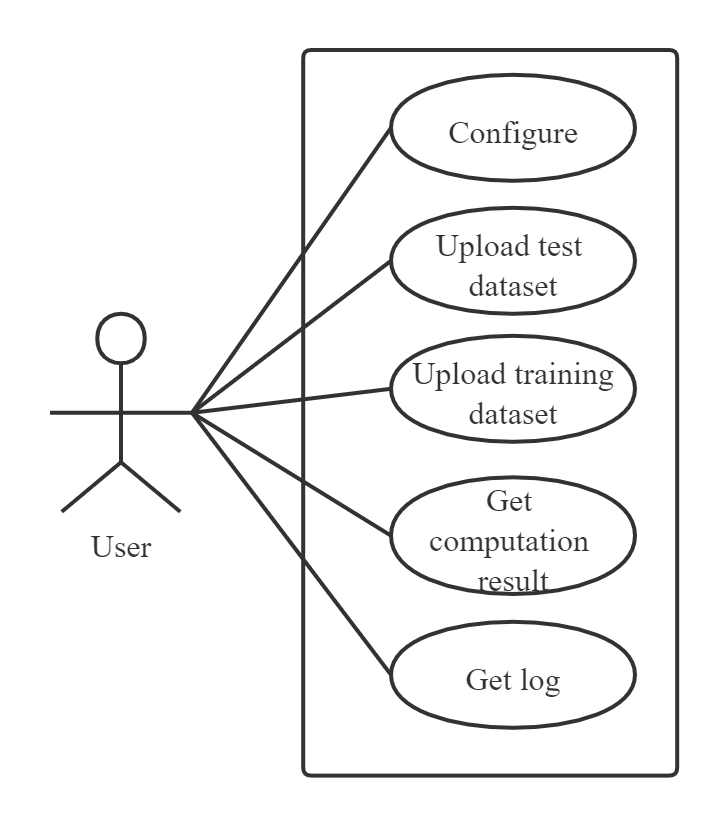
\includegraphics[width=0.75\textwidth]{系统用例图.png}
    \caption{用户用例图}
    \label{fig:badge}
\end{figure}


\section{功能性需求}



功能需求部分主要阐述中文时间表达式信息抽取系统设计所要实现的目标,分析系统各个模块的功能和具体实现方式。本文以用例图直观展示系统需求,以下从用户和开发者角度介绍系统

在中文时间表达式信息抽取系统中,会提供一个用户界面使得用户根据自身需要,选择需要识别的时间数据类型或时间表达式解析后推荐的结果数量,根据选择的配置,下载或导入训练数据与测试数据。

当用户界面将上述的时间数据类型、结果推荐数、训练数据与测试数据导入时间抽取模块之后,时间抽取模块会根据用户导入的或系统默认的训练数据训练时间信息识别模块,当时间信息模块训练完成后,便对用户导入的测试数据进行测试,并通过时间信息归一化模块对识别的结果进行计算。在时间抽取模块的计算过程完成后,会将整体计算结果在用户界面展示,同时用户也可下载日志数据观察详细的计算过程。
同时数据存储层会将用户的训练数据,测试数据,计算结果等保存在数据库中。根据以上分析,可以得出图2中的用例图。

图3-2为系统的开发者用例图,针对开发者而言需要设计中文时间表达式识别和解析两个模块,同时需要配置用户服务接口。
针对识别和解析部分, 我们还需要另外补充朴素贝叶斯选择器模块辅助识别和解析模块以消除中间过程可能产生的歧义问题.
对于用户界面, 首先需要设计上传功能获取用户传入的直接语料或者文档, 必要情况下还需要使用辅助的文字转化功能, 如OCR功能以识别PDF文档中的文字.
将处理后的预料作为识别和解析模块的输入, 最终产生用户所需要的数据格式.
用户上传的数据以及已有的训练语料都应该存放于数据库之中, 便于开发人员纠错以及再训练.

\begin{figure}[h]
    \centering
    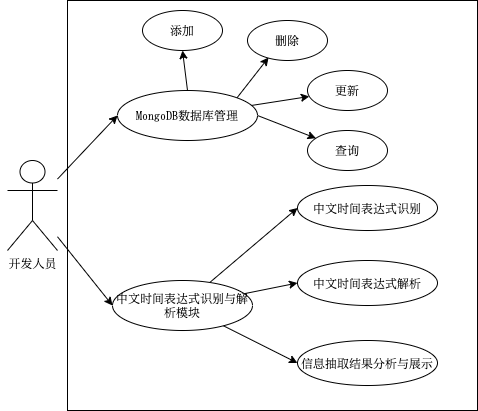
\includegraphics[width=1\textwidth]{开发人员用例.png}
    \caption{开发人员用例图}
    \label{fig:badge}
\end{figure}

\subsection{中文时间表达式识别模块}

中文时间表达式识别模块是为了从文档或语料中获取相关的实体, 并标名实体在语料中的范围, 因此识别模块的功能需求如下所示:
\begin{enumerate}
    \item[(1)] 模块输入不仅能支持普通的文本类型输入, 还需要支持PDF文档以及图片或图片格式的PDF文档, 并且输出为文本形式;
    \item[(2)] 模块必须要准确无歧义的识别到具体的实体, 并以区间的形式标明时间表达式在语料中的具体位置.
\end{enumerate}

\subsection{中文时间表达式解析模块}

中文时间表达式解析模块是根据从识别模块中获取到的实体及实体范围等信息, 解析成UTC时间格式, 方便其他任务需要.
因此中文时间表达式解析模块的功能性需求如下所示:
\begin{enumerate}
    \item[(1)] 将识别到的实体转换为UTC时间格式, 并返回给用户;
    \item[(2)] 为了便于用户理解, 需要将实体解析过程中形成的解析树以可视化的形式呈现给用户;
    \item[(3)] 除了返回最终的UTC时间格式的结果, 还需要提供时间解析的备选方案给用户, 方便用户及时反馈并纠错;
\end{enumerate}

\subsection{相关接口}

对于用户来说,不会关心模型的中间处理步骤,只会关系模型的输出结果,因此为了使用户方便得到结果,需要相关接口进行数据可视化,那么需要满足以下要求:
\begin{enumerate}
    \item[(1)] 输出数据的通用化, 对于用户输入, 若其形式为图片或PDF文档, 应该返回文本形式的语料, 并附上相应的信息, 包括识别到的时间表达式, 时间表达式在语料中的具体位置, 以及时间表达式归一化为UTC时间格式后的字符串, 并将返回数据组织为文档形式, 方便用户下载;
    \item[(2)] 若用户是通过单句预料输入的, 则输出数据的中间结果需要可视化为树形结构, 并在用户界面展示;
    \item[(3)]  用户调用,对于系统的使用,需要规定相关的接口,对服务器进行配置,通过网络请求返回结果。
\end{enumerate}

\section{非功能性需求}

中文时间表达式信息抽取模块在满足功能需求的基础之外, 还需要根据具体的使用情况, 满足非功能性方面的需求.
对于中文时间表达式信息抽取系统应用的非功能需求, 体现在系统的准确性, 系统的实施性, 系统的可扩展性和系统的可维护性.
任何一个软件想要持续的生存下去, 这些性能指标都是不可获取的. 只有同时满足功能性需求和非功能性需求, 该中文时间表达式信息抽取系统才是完整的.

\subsection{准确性}

本中文时间表达式信息抽取系统的准确性是决定项目价值的最重要的因素. 
无论是识别模块还是解析模块的那一部分出错, 都会造成最终结果的不准确, 导致大量的遗漏或者错误解析. 
这样的情况下, 中文时间表达式信息抽取系统将不再具有任何意义.
识别结果的遗漏会显著降低识别模块的可信力, 链式的减少解析模块对最终结果的掌握权, 用户对于中文时间表达式信息抽取结果的全面性会缺乏信任;
错误解析会带来更严重的后果, 如果将某些不属于时间表达式的部分语句解析成正确的结果, 或者无法正确分析时间表达式并将其输出结果, 那么整个系统产生的是反作用:
不仅会让用户对结果感到迷惑, 也对开发人员的错误处理过程造成极大的干扰. 
参考多篇文献及相关的工程项目或开源项目, 本中文时间表达式信息抽取系统要求识别过程应该至少达到90\%, 而解析准确度在识别成功的基础上, 应该至少达到85\%.

\subsection{实时性}

对于本中文时间表达式信息抽取系统的实时识别与解析功能来讲, 优质的交互性体验也是重要的一环. 
这就要求本中文时间表达式信息抽取系统从接收用户输入, 再经过识别与解析, 最后生成可视化视图返回用户的时间应该尽可能处于较短的水平了, 使整个交互过程满足用户的接受范围之内.
因此, 本项目需要对整个处理过程的响应时间进行一定地控制. 因此本项目在本地上进行单句语料的信息抽取时间控制在毫秒级别. 
在远程调用的场景下, 由于需要依赖额外的服务器资源的支持, 尽可能将单句语料的信息抽取时间控制在毫秒到秒级别. 
随着语料内容量级性的增长, 最终的响应时间控制为成线性增长.

\subsection{可扩展性}

中文时间表达式的识别模块根据SCATE标注形式, 定义了许多基本的识别元素, 这些基本的元素相互独立, 耦合性较低. 
在添加新的识别规则时, 开发人员可以根据这些基本的识别元素相互组合, 也可以定义新的基本元素, 当元素或者组合元素与原有的识别规则冲突时, 
识别模块会自动的报道相关的规则冲突.
中文时间表达式的解析模块则是重用了上述的识别元素, 不需要额外开发, 在自动解析过程中动态的组合这些元素. 
因此本中文时间表达式信息抽取系统的可扩展性是良好的, 后续本中文时间表达式信息抽取系统的优化也很好的验证这一点.


\subsection{可维护性}

软件开发过程并不是一蹴而就, 一劳永逸的. 项目初步完成之后, 还需要经历多个版本的迭代, 验证, 再迭代. 
后续开发过程仍然需要不断的维护, 才能保证软件本身的稳定性和可用性.
在本中文时间表达式信息抽取系统的开发中,规则和基本元素的开发人员需尽量使其互相之间是独立的。
本项目的代码需保证组件之间耦合程度低,接口清晰简单,利于后续的维护工作。其次,保证系统模块清晰、代码整洁度高、可读性强、没有冗余代码。
并且全面详细的说明书文档同样有利于软件的维护。

\subsection{可兼容性}

兼容性也是评价一个软件非功能性需求的一个重要指标, 软件具有良好的兼容性才能部署到各种平台, 从而拥有广泛的使用群体; 同时良好的兼容性也避免了项目部署到服务端造成的差异化问题.
如果软件只局限于某一个平台下使用, 显然会限制本中文时间表达式信息抽取系统的用户范围. 本代码在实现语言上依赖于Python, 而工具包仅依赖于scikit-learn. 
并且所有的需求环境全部打包到容器中国呢, 能够同时支持在Linux操作系统和Windows操作系统上部署并稳定运行. 
用户可以通过RESTFul的风格传入语料, 在自己熟悉的环境下使用本中文时间表达式信息抽取系统. 本系统保证良好的兼容性.

\section{本章小结}

本章节从实际需求出发, 根据该中文时间表达式信息抽取系统的应用场景, 详细分析了该信息抽取系统的功能性需求以以非功能性需求.
在功能需求方面, 本章节详细描述了该系统的主要功能, 即本项目需要实现中文时间表达式的识别与解析两种功能. 
同时为了提高用户体验, 另外设计了可视化的树形解析结果, 帮助用户和开发人员校验解析结果的可行性.
在非功能性需求方面, 本系统着重于准确性与实时性两点, 进行了详细的分析. 
为了软件的可持续发展, 又阐述了中文时间表达式信息抽取系统在可兼容性, 可扩展性, 可维护性等方面的具体需求.
本咋给你讲诶对中文时间表达式信息抽取系统的功能性以及非功能性需求, 为下文中的概要设计建立了良好的基础.


% !TeX root = ../main.tex
% HLD: high level design


\chapter{概要设计}

上一章对本中文时间表达式信息抽取系统进行了详尽的需求分析,明晰了该中文时间表达式信息抽取系统需要实现的功能及其他的性能要求。
本章节将基于在第三章中分析所得的功能性需求和非功能性需求,对本中文时间表达式信息抽取系统进行概要设计,并且对该中文时间表达式信息抽取系统的整体架构以及各个模块的功能设计进行详细阐述。
通过该章节的工作内容,读者可以从总体上了解整个系统的设计思路。
本章节的工作为后续详细设计与实现做准备。

\section{系统整体架构设计}

\begin{figure}[h]
  \centering
  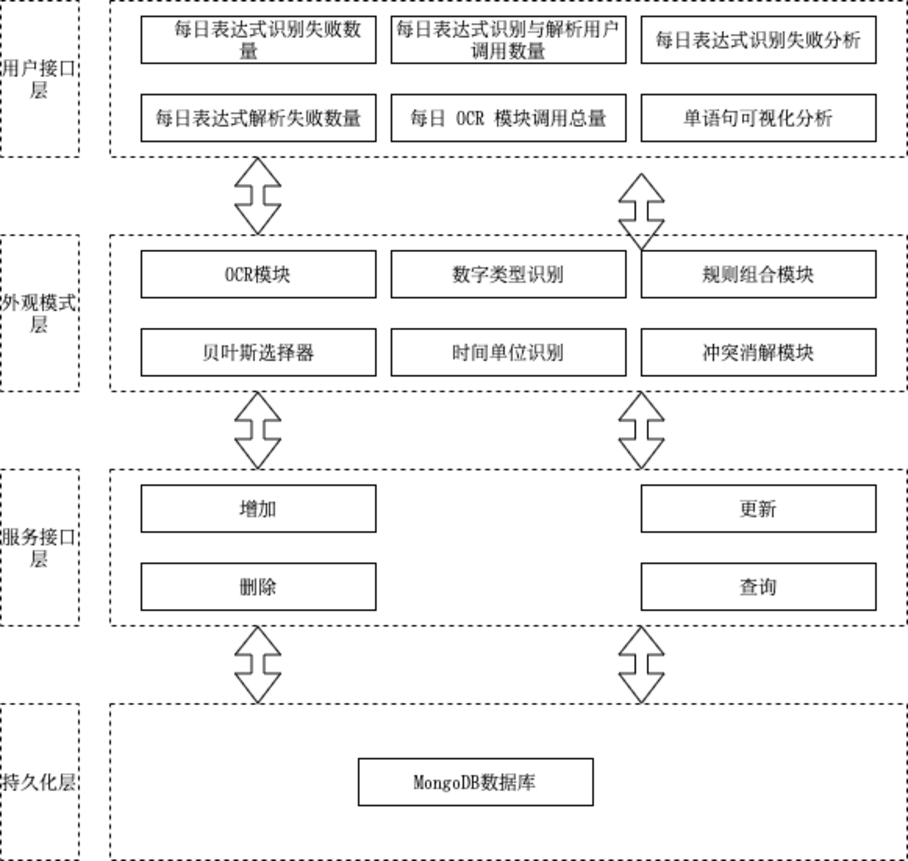
\includegraphics[width=1\textwidth]{系统架构.pdf}
  \caption{系统架构}
  \label{fig:architect}
\end{figure}

由于笔者所在企业的开发要求,软件系统的整体体系架构采用的是浏览器-服务器体系结构,即B/S(Browser/Server)架构,通过基于B/S架构的SaaS(Soft as a Service)平台和Web接口向用户提供服务。
其中浏览器界面负责与客户的信息交互,在运行时间表达式的识别和解析之前,负责获取用户输入的语料和相关的配置等。
服务器后端开发则采用的是典型的四层架构模式,分别为用户接口(API,Application Programming Interface)层,外观(Facade)模式层,服务(Service)层,数据访问(DAO,Data Access Object)层。详情见图4。1。

用户接口层是服务器端与浏览器端进行数据传输的第一站,用户接口层不做过于复杂的逻辑处理,只是将系统内部提供给用户的功能暴露在外,方便与用户交互或被开发人员调用。
在用户接口层承接网络中传入的数据,并将其用系统内部的数据结构封装,传递给外观模式层。

外观模式层是整个服务器后端的业务逻辑核心,可以认为是业务逻辑层。外观模式旨在获取用户接口封装的数据结构并将其解包。
由之前的需求分析可知,用户不仅可以通过用户界面传入单条语句或者多条语句对中文时间表达式信息抽取系统做可行性的检验,以观察系统的输出结果,
也可以传入容量较大的文档、图片以及PDF文档。这时需要使用辅助的OCR模块对用户输入做相应的处理。将非文字的形式转变为系统可以接受的字符串形式。
在解包用户输入以及对用户输入做预处理后,这些数据将被中文时间表达式识别模块接收。
中文时间表达式模块会根据底层的基本元素组合出规则,通过规则匹配的形式将中文时间表达式这一类实体从原语料中提取出来,然后将其抽象化为特殊的元素形式,最后将这些元素提交给中文时间表达式解析模块。
中文时间表达式解析模块将识别模块识别出的元素作为叶结点,自下而上的构建出一棵或多棵语法树,当出现多棵语法树时,将通过朴素贝叶斯选择器模块进行辅助,判断决策采用哪一棵树作为最终的结果树。
结果树在解析的过程中会自然地携带结构化的时间信息,最终在根结点格式化为UTC形式的时间。

服务层主要负责和数据库交互的服务逻辑,负责将外观模式层的处理结果最终保存到数据库中进行持久化。
如果没有服务层作为数据库与业务逻辑之间的桥梁,那大量有价值的原始语料或解析结果将不复存在。
因此,服务层会对数据库中的操作进行简单的聚合,完成较为复杂的数据存取操作。

数据访问层是对数据库表中行记录的具现化,是对象关系映射模型(ORM,Object Relation Mapping)的具体实现,
数据访问层详细的表示了数据库中存储的行记录中各个字段或属性的名称以及类型。
为服务层针对数据库表的操作提供了一定的便捷性。

此外,为了方便用户进行批处理,即传入大量的文档或图片。本中文时间表达式信息抽取系统采用分布式的方法来优化批处理任务。
系统内部一共部署了六台逻辑服务器,其中三台运行中文时间表达式信息抽取系统,用作任务服务器,一台服务器专做数据库服务器,以存储中间数据,一台服务器作为静态资源服务器,一台服务器作为反向代理服务器。
三台任务服务器都使用多线程的方式运行中文时间表达式信息抽取系统。代理服务器采用负载均衡的方式将用户请求产生的负载较为均匀的分配在三台任务服务器上,使得批处理的时间大大剪短。
中文时间表达式信息抽取系统的网络拓扑图如~\ref{fig:network_top}所示。

\begin{figure}[h]
  \centering
  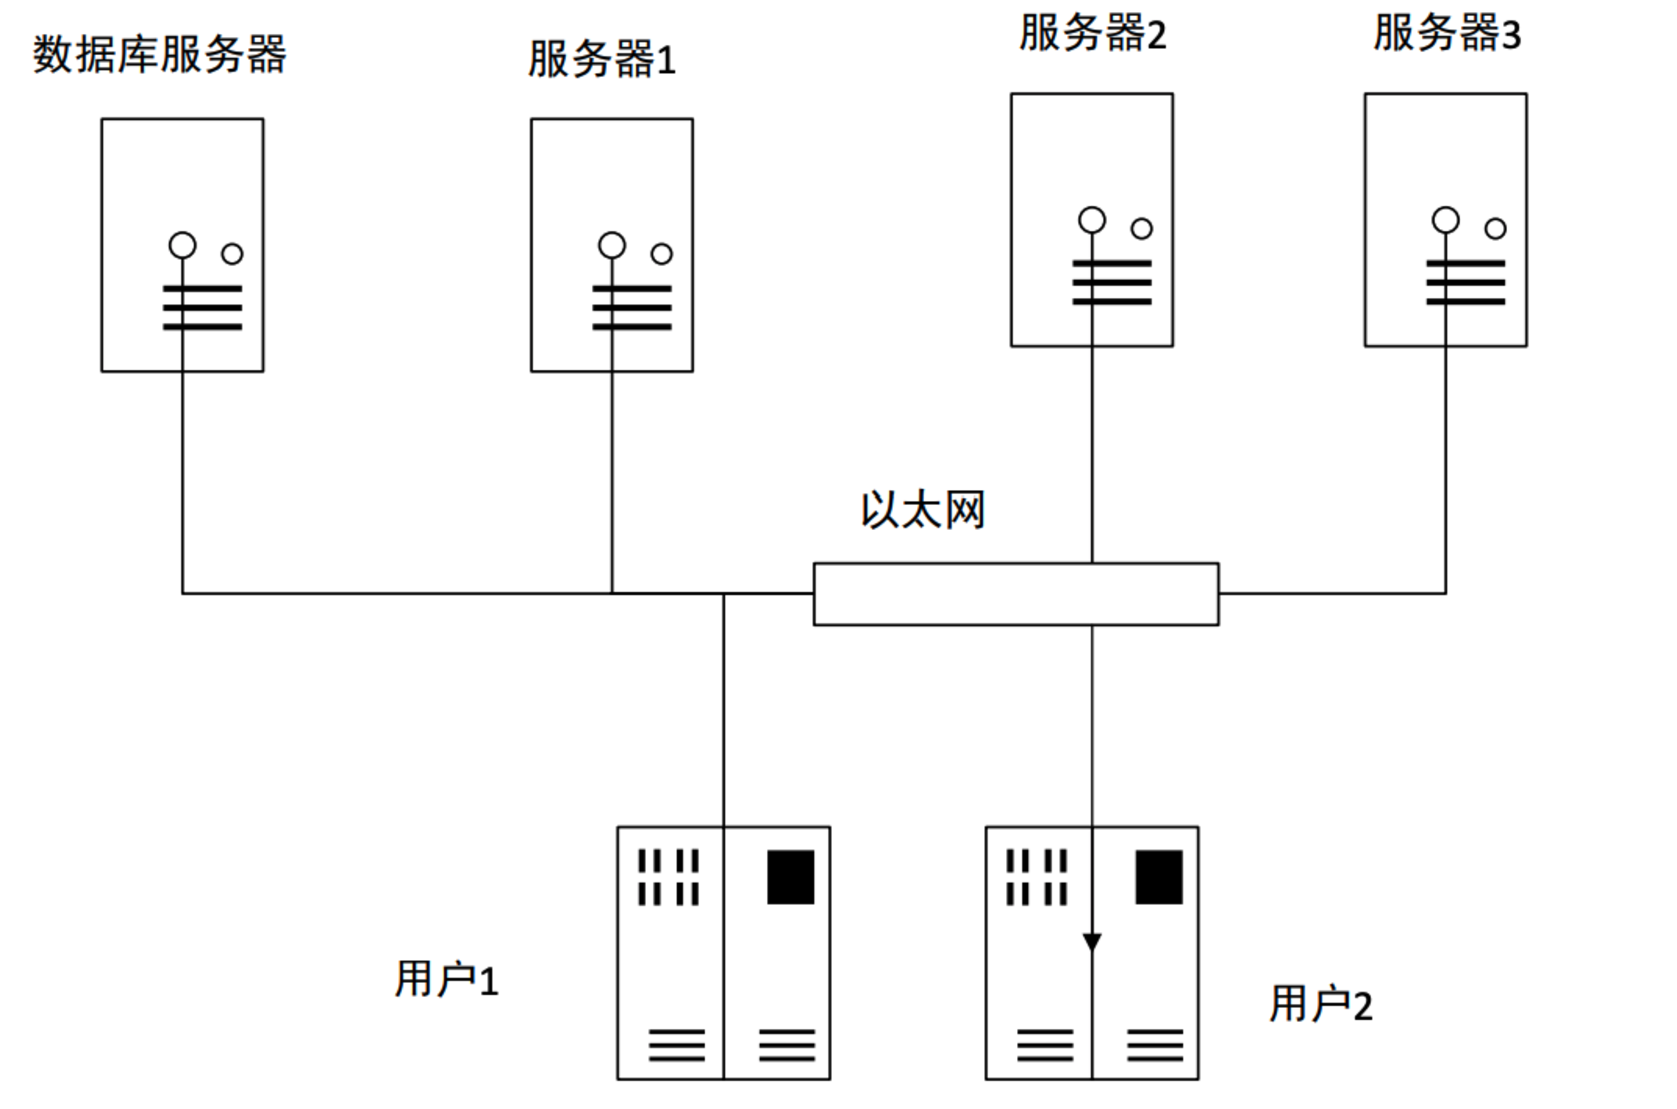
\includegraphics[width=0.7\textwidth]{网络top图.pdf}
  \caption{网络拓扑图}
  \label{fig:network_top}
\end{figure}

\section{系统功能模块设计}

% TODO: 重写该段
中文时间表达式信息抽取系统的功能结构主要依据于模块内部高度集聚的原则,每个模块之间的连接性不高,
类似于固有的制作软件要求,将相互管理的模块进行合并,再对数据进行转换。
在系统内部,并未划分一个独立的方面来进行数据的交流转换,在这样的区别之后,能够更加方便的完成吸引的功能,
按照每个方面彼此之间的关联,可以使各个子系统分层次进行制作和开发,以调用的形式来完成每个模块的要求。
功能模块设计利用系统整体架构设计中提到的用户接口层、外观模式层、服务层、数据访问层四者间的联系来对子系统进行划分。
在单独制作模块的过程中,使用单独的制作来完成功能,确保每个用户功能的独立性,
不会因为极小的变动就会影响全局,使系统的更新和改善互相独立,进而保证系统的安全性。
使用模块的划分来展示系统的作用来进行相应的开发。

\begin{figure}[h]
  \centering
  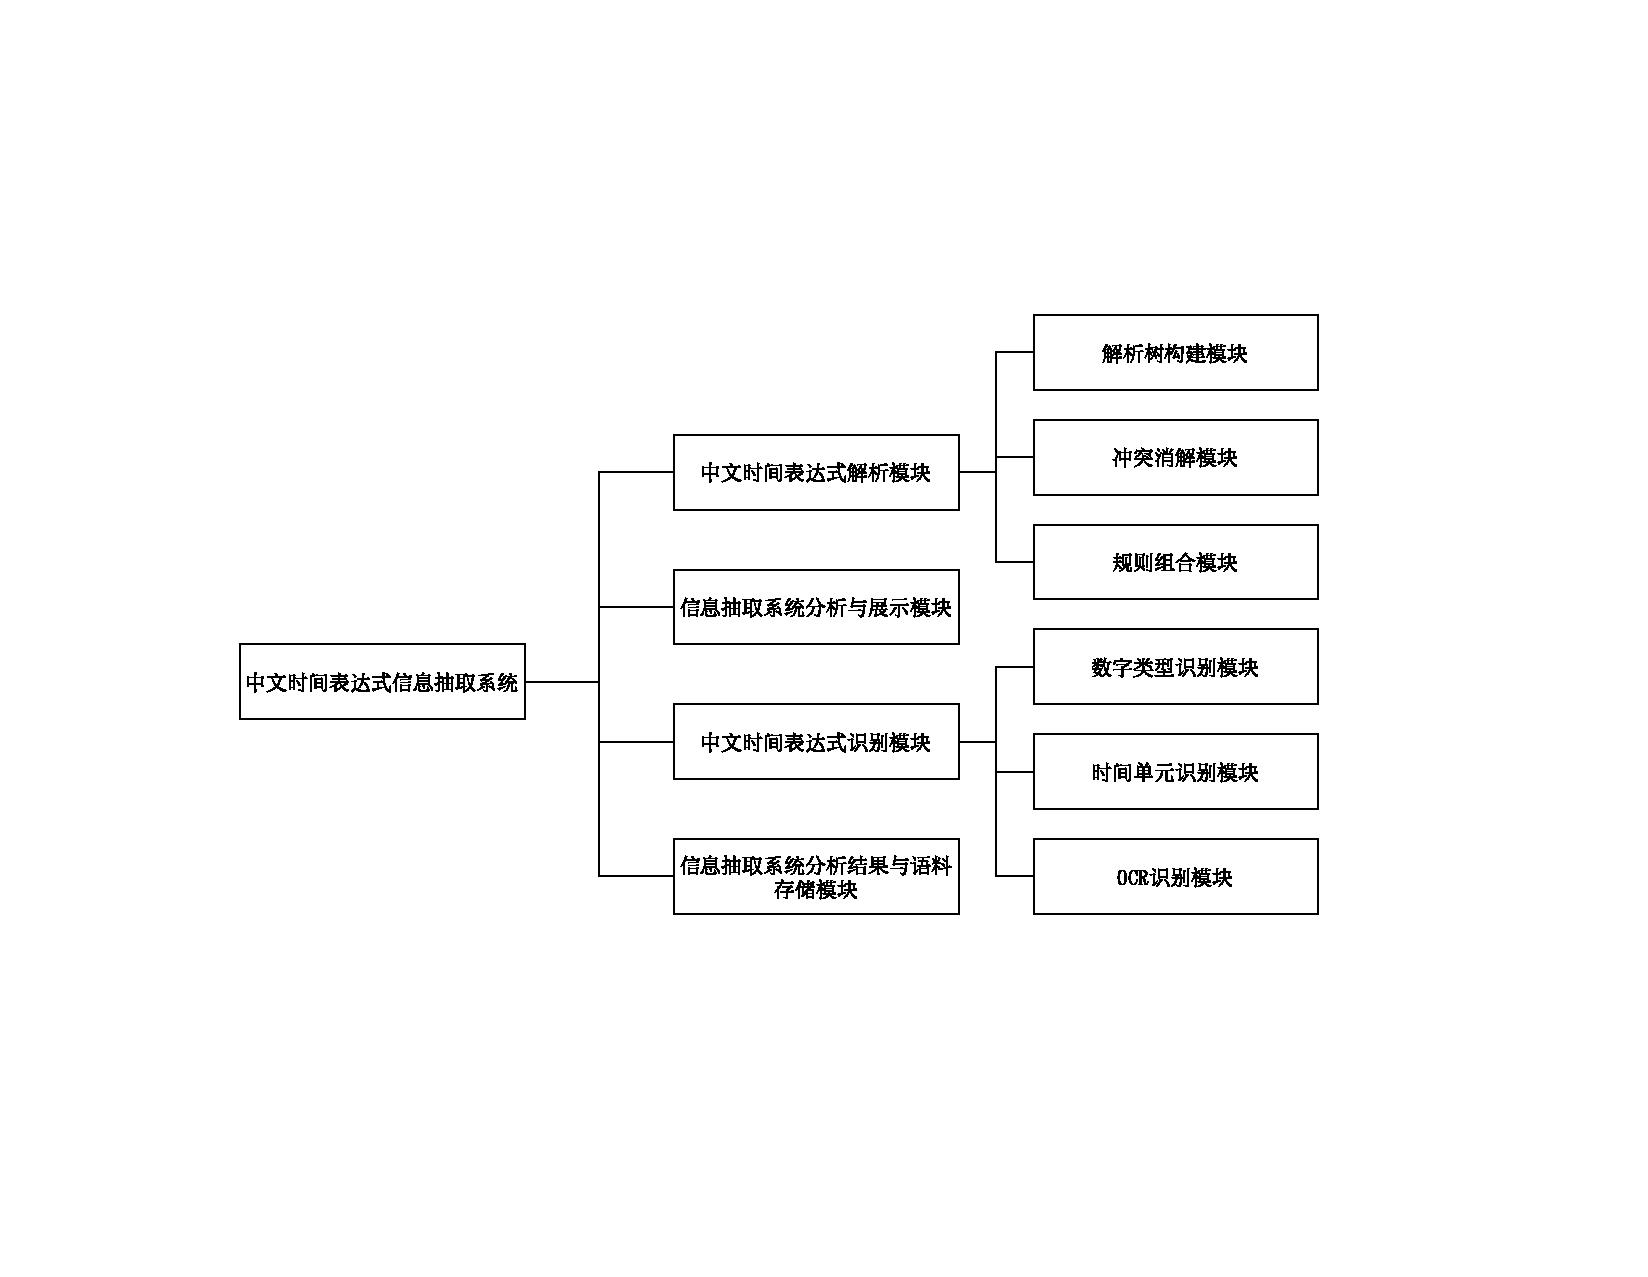
\includegraphics[width=0.9\textwidth]{系统功能模块.pdf}
  \caption{系统功能模块图}
  \label{fig:system_feature}
\end{figure}

\subsection{中文时间表达式识别模块}

当用户进入浏览器中,系统用户界面会默认给用户提供输入为普通文本的选项。如果用户需要修改自己的输入为PDF文档或者图片时,可以显示的将输入修改为PDF文档或图片。
中文时间表达式识别模块在接收到上层用户接口传入的封装数据后,将会根据文件本身的格式和用户选择的输入配置决定对文件的解析方式。如果解析成功则顺利进入下一步识别的流程。
否则将会单独标识文件处理错误,并向用户告知这一文件解析方式存在问题,提醒用户更改输入配置。
如果文本类型为JSON,CSV或TXT格式,那么将会直接进入后续的文本预处理流程。
在根据文件格式和用户输入配置得知文件类型为PDF文档或图片格式时,中文时间表达式识别模块将该文件委托给OCR识别模块进行识别。识别的结果将会返回后续的文本预处理流程。
在初步得到文本文件后,需要使用与文本预处理模块对文本中含有的表情,全半角符号或者转义符号做一定的处理,防止后续的识别过程识别到错误的实体。
当文本文件经过预处理后,将会同时被数字类型识别模块和时间单元识别模块同时处理。
数字类型识别模块将通过正则匹配的形式匹配到文本中所有的中文或英文数字,并将其封装成数字类型基本元素对象。
而时间识别单元也是通过正则匹配的形式匹配到文本中所有的中文形式的时间单元,并将其封装为时间类型基本元素对象。
这些识别到的对象会根据在文本中出现的顺序进行排序,并交付给中文时间表达式解析模块进行解析。

\subsection{中文时间表达式解析模块}

如果系统内部还没有朴素贝叶斯选择器的模型参数,将会首先读取语料库中的所有语料,根据事先已经标注好的训练集做简单的预料训练。
中文时间表达式解析模块首先将系统内部定义好所有基本元素对象按照事先已经定义好的规则进行组合,然后调用上文中所述的中文时间表达式识别模块进行识别。
规则识别模块将识别出的基本元素需要按照上下文无关语法的产生式进行反向推到,用以得到所有的推导规则。
统计每一个推导规则在整个语料中识别出的所有规则的概率值,以此值作为似然记录下来。待到所有的推导规则似然值的统计完毕,即可组建似然函数。
此后解析树构建模块按照概率无关上下文语法将,通过中文时间表达式识别模块的得到的用户输入产生的基本元素,通过规则组合模块处理得到的一系列规则,
按照每个规则的似然值,自下而上的构建出一棵或多棵语法树。
如果在构建树的过程中出现了冲突,那么冲突消解模块会根据似然函数进行冲突消解。

\subsection{信息抽取系统分析结果与语料存取模块}

信息抽取系统分析结果与语料存取模块主要负责中文时间表达式信息抽取系统中将分析结果和语料存入到数据库中。
用户传入的语料首先会生成对应的序列号,进行唯一标识,然后存入数据库中。
如果用户传入的类型为PDF文档类型或图片类型,则为文件资源生成唯一标识码,并将该文件类型重命名为唯一标识码,存放到系统指定位置。
随后语料会经过识别和解析两个模块,生成最终的结果。
信息抽取系统分析结果与语料存储模块将该结果按照序列号存入对应的行记录中,此时需要按照开发人员提前配置好的文件,决定最终录入数据库中数据的大小。
最终结果需要包含识别到的实体,实体边界还有相应的语法分析树。
当开发人员需要读取语料或者用户需要分析结果,此时信息抽取系统分析结果与语料存取模块需要读取用户传入或开发人员定义好的配置,从数据库中取出相应的数据,
交付给信息抽取系统分析与展示模块进行展示。

\begin{figure}[h]
  \centering
  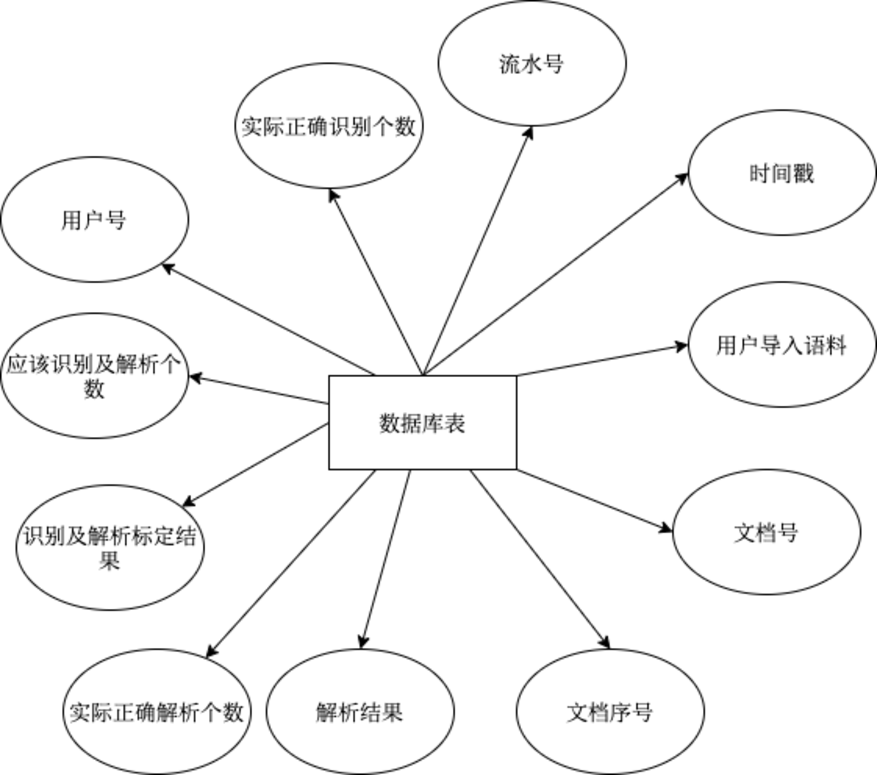
\includegraphics[width=0.8\textwidth]{er.pdf}
  \caption{ER图}
  \label{fig:er_graph}
\end{figure}

\subsection{信息抽取系统分析与展示模块}

信息抽取系统分析与展示模块通过Metis面板读当前数据分析需求向后台的MongoDB数据库进行SQL语句查询请求,并且将查询结果以可视化的方式显示到Metis面板智商。
当前改模块一共进行10个查询需求,下面对每一项功能进行详细的说明。

\begin{enumerate}
  \item[(1)] 每日表达式识别失败数量

    每日表达式识别失败数量查询需求可以通过在数据库表的时间戳字段上建立索引,并且通过查询数据库表上每个行记录识别失败总量之和,即可得出每日表达式识别失败总量。

  \item[(2)] 每日表达式解析失败数量

    每日表达式解析失败数量查询需求可以通过在数据库表的时间戳字段上建立索引,并且通过查询数据库表上每个行记录解析失败总量之和,即可得出每日表达式解析失败总量。

  \item[(3)] 每日表达式识别与解析用户调用数量

    每日表达式识别与解析用户调用数量查询需求可以通过在数据库表的时间戳字段和用户唯一标识字段建立索引,并且通过查询数据库表上当天每用户查询总量,即可得出每日表达式识别与解析用户调用数量。

  \item[(4)] 每日OCR模块调用总量

    每日OCR模块调用总量可以通过在数据库表的时间戳字段上建立索引,并且根据行记录的文件类型是否为PDF文档或图片类型进行计算,即可得出每日表达式识别与解析用户调用数量。

  \item[(5)] 每日表达式识别失败分析

    每日表达式识别失败分析可以通过在数据库表的时间戳字段上建立索引,并且根据行记录中的失败记录和中文时间表达式解析树进行分析,即可得到每日表达式识别失败分析。

  \item[(6)] 每日表达式解析失败分析

    每日表达式识别失败分析可以通过在数据库表的时间戳字段上建立索引,并且根据行记录中的失败记录和中文时间表达式解析树进行分析,即可得到每日表达式识别失败分析。

  \item[(7)] 单语句可视化分析

    单语句可视化分析可以通过在数据库表的时间戳字段上建立索引,并且根据行记录中的中文时间表达式解析树进行分析,即可得到单语句可视化分析。
\end{enumerate}

\begin{table}[h]
  \centering
  \caption{数据库表结构设计}
  \begin{tabular}{|*{7}{c|}}
    \hline
    序号 & 字段名          & 字段说明                 & 类型    & \makecell*[c]{是否                                              \\为空} & 说明                  & 默认值        \\
    \hline
    1    & uid             & 用户号                   & String  & 否                 & \makecell*[c]{PK(uid,sid,              \\doc\_id)} & “0”           \\
    \hline
    2    & sid             & 流水号                   & String  & 否                 & \makecell*[c]{PK(uid,sid,              \\doc\_id)} & “0”           \\
    \hline
    3    & create\_date    & 创建时间戳               & Date    & 否                 & null                       & CURRENT\_DATE \\
    \hline
    4    & doc             & \makecell*[c]{用户                                                                                   \\导入语料} & String  & 否       & null                  & “0”           \\
    \hline
    5    & doc\_id         & 文档号                   & String  & 否                 & \makecell*[c]{PK(uid,sid,              \\doc\_id)} & “0”           \\
    \hline
    6    & doc\_num        & 文档序号                 & Integer & 否                 & null                       & "0"           \\
    \hline
    7    & result          & 解析结果                 & String  & 否                 & null                       & “0"           \\
    \hline
    8    & real\_num       & \makecell*[c]{应该识别                                                                               \\及解析个数} & Integer & 否 & null & 0 \\
    \hline
    9    & resolution\_num & \makecell*[c]{实际正确                                                                               \\解析个数} & Integer & 否 & null & 0 \\
    \hline
    10   & reconition\_num & \makecell*[c]{实际正确                                                                               \\识别个数} & Integer & 否 & null  & 0 \\
    \hline
    11   & label           & \makecell*[c]{识别及解析                                                                             \\标定结果} & String & 否 & null & “0” \\
    \hline
  \end{tabular}
\end{table}

\section{数据库设计}

数据库是本系统的重要组成部分,主要负责中文时间表达式信息抽取系统中导出数据的持久化存储方面的工作。
数据库及相关数据表的设计也是软件开发工程里设计流程中非常关键的步骤之一,因为数据库的设计关系到上层查询接口的易用性,查询效率以及数据的完整性和一致性,是保障数据存储效率和数据完整安全的重要环节。
因为中文时间表达式信息抽取系统大量的使用文本类型数据,数据的JSON化程度较高。在当前众多的开源数据库中,非关系型数据库(NoSQL,Not-only SQL)是比较适合存储这类大文本类型的数据的。
其中MongoDB又是特意为文本存储设计的键-值对数据库,是一款拥有高兴能的数据库管理系统,
因此本中文时间表达式抽取系统底层采用MongoDB进行数据持久层的开发。

\section{本章小节}

本章节主要从中文时间表达式信息抽取系统的整体设计入手,详细介绍了本信息抽取系统的整体架构。
信息抽取系统主要分为四个模块: 信息抽取系统分析结果与预料存储模块,中文时间表达式识别模块,中文时间表达式解析模块以及信息抽取系统分析与展示模块,并分别对上述模块的功能进行了阐明,设计并展示了各个子模块的活动图。
其中中文时间表达式识别和解析模块内部又存在多个相辅相成,互相作用的子模块。本章内容详细介绍了本信息抽取系统的整体设计以及功能模块设计。
最后,本系统还使用了数据库存储系统用以存取解析结果,对解析结果的数据结构及其春初进行了设计。本章的概要设计工作为本中文时间表达式信息抽取系统的详细设计与实现提供了方向。

% !TeX root = ../main.tex
% LLD: Low Level Design

\chapter{详细设计与实现}

本章节主要在概要设计的基础之上, 对本中文时间表达式信息抽取系统的详细设计给出具体解决方案并进行实现, 其内容主要包括各个模块的详细设计和逻辑实现.
本章节深入理解概率无关上下文语法的原理及其工作的上下文环境, 设计实现各种识别和解析规则, 完成本中文时间表达式信息抽取系统的编码实现.

\section{模块设计与实现}

\subsection{中文时间表达式识别模块的设计与实现}

\subsubsection{中文时间表达式识别的概率无关上下文语法定义}

中文时间表达式的识别和解析都是以概率无关上下文语法为核心算法实现的.
对于中文时间表达式, 涉及到两个比较关键的部分, 一部分是对数字部分的识别, 另一部分是对时间单元的识别, 最后是有机的将这些识别规则组合到一起.
概率无关上下文语法通常四元组的形式出现: (N, R, S,  $\varSigma$). 其中N代表的是非终止符号集合, $\varSigma$ 代表的是终止符号的集合, $\varSigma$.
R代表的是一规则或者是产生式的结合, 对于每一个产生式, 其组成形式应该为 A $\rightarrow$ $\beta$[p], 其中A应该为一个非终止符, beta是一个包含0个或多个符号的字符串,
字符串的形式应该为($\varSigma$ $\cup$ N), 即非终结符与终结符的交集中产生的字符串. p则为一个介于0和1中间的数字, 表示 P($\beta$|A)的概率.
P($\beta$|A)可以理解为由终止符产生相应的表达式字符串的概率, 即该产生式的概率.
S则为其实符号.

其中部分与中文整数相关的终止符定义如下:

\begin{table}[h]
    \centering
    \caption{部分中文整数终止符}
    \begin{tabular}{*{4}{c}}
        \toprule
        类名                  & 描述                                                                         & 蕴含字符                       & 对应数字                          \\
        \midrule
        CHINESE\_DIGITS       & 简体中文数字                                                                 & \makecell*[c]{〇,一, 二,三,四,                                     \\ 五,六,七,八,九} & \makecell*[c]{0, 1, 2, 3, 4, \\ 5, 6, 7, 8, 9}         \\
        CHINESE\_DIGITS\_TRAD & 繁体中文数字                                                                 & \makecell*[c]{零,壹,贰,叁,肆,                                      \\ 伍,陆,柒,捌,玖}  & \makecell*[c]{0, 1, 2, 3, 4, \\ 5, 6, 7, 8, 9}         \\
        CHINESE\_UNITS        & \makecell*[c]{简体中文                                             数字单位} & \makecell*[c]{十, 百, 千,                                          \\ 万, 十万, 百万}     & \makecell*[c]{$10^1, 10^2, 10^3,$ \\ $10^4, 10^5, 10^6$} \\
        CHINESE\_UNITS\_TRAD  & \makecell*[c]{繁体中文                                             数字单位} & 拾,佰,仟,萬,億                 & \makecell*[c]{$10^1, 10^2, 10^3,$ \\ $10^4, 10^8$}       \\
        \bottomrule
    \end{tabular}
\end{table}


部分与阿拉伯整数相关的终止符相关的终止符定义如下

\begin{table}[h]
    \centering
    \caption{部分中文整数终止符}
    \begin{tabular}{*{4}{c}}
        \toprule
        类名         & 描述       & 蕴含字符                     & 对应数字     \\
        \midrule
        ArabicDigit  & 阿拉伯数字 & \makecell*[c]{0, 1, 2, 3, 4,                \\ 5, 6, 7, 8, 9} & \makecell*[c]{0, 1, 2, 3, 4, \\ 5, 6, 7, 8, 9}         \\
        MIXED\_SIGNS & 正负符号   & 正, +, 负, -                 & 1, 1, -1, -1 \\
        \bottomrule
    \end{tabular}
\end{table}

\subsubsection{预处理过程}

在钱文忠已经给出定义与时间表达式相关的终结符(terminal)和非终结符(non-terminals),终结
符在文本匹配中类似于正则表达式,以确定时间表达式的区间(span)。非终结符则在最后对
时间表达式抽象成的语法树中充当非叶结点。图 6 中由终结符和非终结符组成的产生式
(production)最终将被简化为 CNF(Chomsky norm function)。同时我们需要向语料库中写入
语料,语料库中的每条数据应该以(文本,结果)的文本对的形式存储,语料库作为训练集以
求得每个产生式的似然。产生式的似然将参与求得语法树整体概率的计算.

\subsubsection{分析树的构建}

首先需要定义与时间表达式相关的终结符(terminal)和非终结符(non-terminals),终结
符在文本匹配中类似于正则表达式,以确定时间表达式的区间(span)。非终结符则在最后对
时间表达式抽象成的语法树中充当非叶结点。图 6 中由终结符和非终结符组成的产生式
(production)最终将被简化为 CNF(Chomsky norm function)。同时我们需要向语料库中写入
语料,语料库中的每条数据应该以(文本,结果)的文本对的形式存储,语料库作为训练集以
求得每个产生式的似然。产生式的似然将参与求得语法树整体概率的计算

\subsubsection{冲突消解}

如图 9,同一个时间表达式可能解析出多棵语法树,需要最终选择在总概率上为 top-k 的
k 棵语法树,即总体概率最大的 k 棵树。解析树的整体概率为树上所有产生式概率的乘积,在
本项目中将 k 的值设为 1,则最终的语法树的概率如下。S 表示识别到的时间表达式,Tree 为
生成的解析树,n 为树中产生式的数量。


\subsection{中文时间表达式识别模块的设计与实现}

在使用句法分析获得时间表达式的语法树后,我们还需要将整棵树归一化到一种具体的
标注格式,这里我们选择了 SCATE 并加以改良,使其更贴合与中文的时间表达。归一化核心
的数据结构有三:
1) Period:时间轴上的基本时间单位数量之和,如‘3 天’,‘2 个小时 30 分钟’;
2) Interval:时间轴上一段左闭右开的,能确定到年份(year)的区间,如‘2019 年’,
‘2019 年 3 月’;
3) Repeat-interval:时间轴上一段左闭右开的,不包括年份,表示在时间轴上具有重复性
的一段区间,如‘3 月份’,‘5 点 20 分’。
我们以三种数据结构为核心,并用操作符集合(operator set)来表示时间表达式的语义。
在表 4 中列举出部分典型操作符。在构建时间表达式分析树的过程中,其实已经将操作符与数
据结构相结合,分析树构建完成后,树的根结点会将操作符集合形成嵌套表达式保存,直到我
们需要将时间表达式转化为特定的结构化信息时,才进行嵌套表达式的计算,以实现惰性计算
(lazy evaluation)。根结点的最终计算结果应该是以 ISO 格式描述的有起止时间的区间或类似
格式的时间段,如‘2019 年 3 月 2 日’,表达式最终计算的结果应该为‘Interval(start=2019-03-
02T00:00:00, end=2019-03-03T00:00:00)’。

\subsection{时间信息抽取系统分析与展示模块}

\subsubsection{中文时间表达式识别的概率无关上下文语法定义}

中文时间表达式的识别和解析都是以概率无关上下文语法为核心算法实现的.
对于中文时间表达式, 涉及到两个比较关键的部分, 一部分是对数字部分的识别, 另一部分是对时间单元的识别, 最后是有机的将这些识别规则组合到一起.
概率无关上下文语法通常四元组的形式出现: (N, R, S,  $\varSigma$). 其中N代表的是非终止符号集合, $\varSigma$ 代表的是终止符号的集合, $\varSigma$.
R代表的是一规则或者是产生式的结合, 对于每一个产生式, 其组成形式应该为 A $\rightarrow$ $\beta$[p], 其中A应该为一个非终止符, beta是一个包含0个或多个符号的字符串,
字符串的形式应该为($\varSigma$ $\cup$ N), 即非终结符与终结符的交集中产生的字符串. p则为一个介于0和1中间的数字, 表示 P($\beta$|A)的概率.
P($\beta$|A)可以理解为由终止符产生相应的表达式字符串的概率, 即该产生式的概率.
S则为其实符号.

其中部分与中文整数相关的终止符定义如下:

\begin{table}[h]
    \centering
    \caption{部分中文整数终止符}
    \begin{tabular}{*{4}{c}}
        \toprule
        类名                  & 描述                                                                         & 蕴含字符                       & 对应数字                          \\
        \midrule
        CHINESE\_DIGITS       & 简体中文数字                                                                 & \makecell*[c]{〇,一, 二,三,四,                                     \\ 五,六,七,八,九} & \makecell*[c]{0, 1, 2, 3, 4, \\ 5, 6, 7, 8, 9}         \\
        CHINESE\_DIGITS\_TRAD & 繁体中文数字                                                                 & \makecell*[c]{零,壹,贰,叁,肆,                                      \\ 伍,陆,柒,捌,玖}  & \makecell*[c]{0, 1, 2, 3, 4, \\ 5, 6, 7, 8, 9}         \\
        CHINESE\_UNITS        & \makecell*[c]{简体中文                                             数字单位} & \makecell*[c]{十, 百, 千,                                          \\ 万, 十万, 百万}     & \makecell*[c]{$10^1, 10^2, 10^3,$ \\ $10^4, 10^5, 10^6$} \\
        CHINESE\_UNITS\_TRAD  & \makecell*[c]{繁体中文                                             数字单位} & 拾,佰,仟,萬,億                 & \makecell*[c]{$10^1, 10^2, 10^3,$ \\ $10^4, 10^8$}       \\
        \bottomrule
    \end{tabular}
\end{table}


部分与阿拉伯整数相关的终止符相关的终止符定义如下

\begin{table}[h]
    \centering
    \caption{部分中文整数终止符}
    \begin{tabular}{*{4}{c}}
        \toprule
        类名         & 描述       & 蕴含字符                     & 对应数字     \\
        \midrule
        ArabicDigit  & 阿拉伯数字 & \makecell*[c]{0, 1, 2, 3, 4,                \\ 5, 6, 7, 8, 9} & \makecell*[c]{0, 1, 2, 3, 4, \\ 5, 6, 7, 8, 9}         \\
        MIXED\_SIGNS & 正负符号   & 正, +, 负, -                 & 1, 1, -1, -1 \\
        \bottomrule
    \end{tabular}
\end{table}

\subsubsection{预处理过程}

在钱文忠已经给出定义与时间表达式相关的终结符(terminal)和非终结符(non-terminals),终结
符在文本匹配中类似于正则表达式,以确定时间表达式的区间(span)。非终结符则在最后对
时间表达式抽象成的语法树中充当非叶结点。图 6 中由终结符和非终结符组成的产生式
(production)最终将被简化为 CNF(Chomsky norm function)。同时我们需要向语料库中写入
语料,语料库中的每条数据应该以(文本,结果)的文本对的形式存储,语料库作为训练集以
求得每个产生式的似然。产生式的似然将参与求得语法树整体概率的计算.

\subsubsection{分析树的构建}

首先需要定义与时间表达式相关的终结符(terminal)和非终结符(non-terminals),终结
符在文本匹配中类似于正则表达式,以确定时间表达式的区间(span)。非终结符则在最后对
时间表达式抽象成的语法树中充当非叶结点。图 6 中由终结符和非终结符组成的产生式
(production)最终将被简化为 CNF(Chomsky norm function)。同时我们需要向语料库中写入
语料,语料库中的每条数据应该以(文本,结果)的文本对的形式存储,语料库作为训练集以
求得每个产生式的似然。产生式的似然将参与求得语法树整体概率的计算

\subsubsection{冲突消解}

如图 9,同一个时间表达式可能解析出多棵语法树,需要最终选择在总概率上为 top-k 的
k 棵语法树,即总体概率最大的 k 棵树。解析树的整体概率为树上所有产生式概率的乘积,在
本项目中将 k 的值设为 1,则最终的语法树的概率如下。S 表示识别到的时间表达式,Tree 为
生成的解析树,n 为树中产生式的数量。


\subsection{时间信息抽取系统分析结果与语料春初模块}

在使用句法分析获得时间表达式的语法树后,我们还需要将整棵树归一化到一种具体的
标注格式,这里我们选择了 SCATE 并加以改良,使其更贴合与中文的时间表达。归一化核心
的数据结构有三:
1) Period:时间轴上的基本时间单位数量之和,如‘3 天’,‘2 个小时 30 分钟’;
2) Interval:时间轴上一段左闭右开的,能确定到年份(year)的区间,如‘2019 年’,
‘2019 年 3 月’;
3) Repeat-interval:时间轴上一段左闭右开的,不包括年份,表示在时间轴上具有重复性
的一段区间,如‘3 月份’,‘5 点 20 分’。
我们以三种数据结构为核心,并用操作符集合(operator set)来表示时间表达式的语义。
在表 4 中列举出部分典型操作符。在构建时间表达式分析树的过程中,其实已经将操作符与数
据结构相结合,分析树构建完成后,树的根结点会将操作符集合形成嵌套表达式保存,直到我
们需要将时间表达式转化为特定的结构化信息时,才进行嵌套表达式的计算,以实现惰性计算
(lazy evaluation)。根结点的最终计算结果应该是以 ISO 格式描述的有起止时间的区间或类似
格式的时间段,如‘2019 年 3 月 2 日’,表达式最终计算的结果应该为‘Interval(start=2019-03-
02T00:00:00, end=2019-03-03T00:00:00)’。


\section{本章小结}

本章主要介绍了基于概率无关上下文语法的中文时间表达式信息抽取系统的详细设计和实现,
首先从整体描述了系统的架构和各个模块的结构,包括中文时间表达式识别模块的设计与实现、中文时间表达式识别模块的设计与实现、
时间信息抽取系统分析与展示模块的设计与实现、时间信息抽取系统分析结果与预料存储模块的设计与实现.
部分模块还给出了相关时序图和类图详细设计。

% !TeX root = ../main.tex

\chapter{系统测试和分析}

软件测试是软件开发的最后一道程序,软件测试分为功能性测试和非功能性
测试。功能性测试是为了保证需求分析的预期功能都被实现,给用户提供满意的
交付。非功能性测试是为了保证软件的性能及使其实现可持续发展,主要关注于
系统的可维护性、扩展性、健壮性、兼容性等。此外,对于安全性要求较高软件
系统,还需要进行大量的安全性测试,来保证安全性。本文的上一章节介绍了本
中文时间表达式信息抽取系统的详细设计及实现,本章将对实现的中文时间表达式信息抽取系统进行测试,其主
要目的是验证本中文时间表达式信息抽取系统是否能够准确有效的支持中文时间表达式的识别解析,是否能正确的存储到数据库中,是否能正确完成用户界面的渲染。

\section{测试方案}

系统采用单元测试的方式对各个模块的功能函数进行正确性测试,在提供的
测试环境中对系统的各项功能进行功能性测试,对系统整体的性能做性能测试,
最后对测试结果进行详细的分析和总结。主要的测试方案如下:
(1)web 客户端:通过浏览器访问本系统,在 web 页面上的组件上发送各类查询需求,检查返回数据是否完整,页面渲染是否符合预期结果。
(2)服务端:对 web 客户端的查询请求进行解析和检查,检查查询请求是
否都能正确到达服务端,并且被服务端所处理。根据服务端的资源消耗分析系统
的性能瓶颈。
(3)数据库:通过对数据库接口进行测试,检查数据库接口对于指定查询
需求是否能返回数据库中存在的正确数据,数据库对查询请求的响应时间是否具
有可用性。
(4)客户端、服务端以及数据库访问接口模块中的代码做单元测试。

\section{测试环境}

本中文时间信息抽取可以部署在 Linux 和 Windows 系统环境中。在实际的应用
中,Linux较Windows更为稳定,服务部署的方案也更成熟,故将系统部署到Linux的发行版Ubuntu上。

本地测试环境部署实例为1台实例。 本地测试环境见表~\ref{tab:local_test}

\begin{table}[h]
    \centering
    \caption{Linux软件环境}
    \begin{tabular}{|*{3}{c|}}
        \hline
        项目       & 软件               & 版本      \\
        \hline
        操作系统   & Ubuntu             & 18.04 LTS \\
        \hline
        编辑器     & Visual Studio Code & 1.41      \\
        编程语言   & Python             & 3.7.2     \\
        \hline
        代理服务器 & Nginx              & 1.17.2    \\
        \hline
        工具库     & SciKit-learn       & 0.21.1    \\
        \hline
    \end{tabular}
    \label{tab:local_test}
\end{table}

服务端测试环境部署实例为4台实例,其中三台为服务处理实例,一台为MongoDB实例。 服务实例环境见表~\ref{tab:server_test}
\begin{table}[h]
    \centering
    \caption{Linux软件环境}
    \begin{tabular}{|*{3}{c|}}
        \hline
        项目       & 软件               & 版本   \\
        \hline
        操作系统   & CentOS             & 7      \\
        \hline
        编辑器     & Visual Studio Code & 1.41   \\
        编程语言   & Python             & 3.7.2  \\
        \hline
        代理服务器 & Nginx              & 1.17.2 \\
        \hline
        工具库     & SciKit-learn       & 0.21.1 \\
        \hline
        内存       & 8G                 &        \\
        \hline
        CPU        & Intel              & 7900K  \\
        \hline
    \end{tabular}
    \label{tab:server_test}
\end{table}


\section{单元测试}

\subsection{单元测试概述}

单元测试的内容主要对本地部署的服务端实例的正确性进行测试,本系统采用Python语言的pytest单元测试框架进行测试,通过命令行运行pytest测试指令,检查测试结果的正确性。

\subsection{单元测试方案设计}


本地部署的服务端实例的单元测试采用 Python 语言的 pytest 单元测试框架,服务端单元测
试方法主要针对本系统的中文时间表达式信息识别模块,解析模块以及数据库持久化存储的接口,单元
测试对模块中出现的所有功能函数可能出现的错误或者异常结果进行测试和路
径覆盖,主要的测试用例如下表~\ref{tab:unit_test} 所示。

\begin{table}[h]
    \centering
    \caption{单元测试方案表}
    \resizebox*{\linewidth}{!}{
        \begin{tabular}{|*{4}{c|}}
            \hline
            测试项                         & 测试步骤                             & 预期结果 & 实际结果 \\
            \hline
            \makecell*[c]{中文时间表达式                                                                \\ 信息抽取模块 \\配置加载失败} & \makecell*[c]{1. 构造中文时间表达式\\信息抽取模块\\配置文件参数,\\使得某些\\重要参数缺失;\\2. 启动中文时间表达式\\信息抽取模块。} & \makecell*[c]{中文时间表达式\\信息抽取模块\\启动失败} & \makecell*[c]{中文时间表达式\\信息抽取模块\\启动失败} \\
            \hline
            \makecell*[c]{中文时间表达式                                                                \\信息抽取模块\\配置加载异常} & \makecell*[c]{1. 构造中文时间表达式\\信息抽取模块\\配置文件参数,\\在配置文件中\\设置错误的参数类型;\\2. 启动中文时间表达式\\信息抽取模块。} & \makecell*[c]{中文时间表达式\\信息抽取模块\\启动失败} & \makecell*[c]{中文时间表达式\\信息抽取模块\\启动失败} \\
            \hline
            \makecell*[c]{中文时间表达式                                                                \\信息抽取模块\\配置加载成功} & \makecell*[c]{1. 构造中文时间表达式\\信息抽取模块\\配置文件参数,\\给予配置文件中\\正确的配置参数;\\2. 启动中文时间表达式\\信息抽取模块。} & \makecell*[c]{中文时间表达式\\信息抽取模块\\启动成功} & \makecell*[c]{中文时间表达式\\信息抽取模块\\启动成功} \\
            \hline
            \makecell*[c]{中文时间表达式                                                                \\信息抽取模块\\文本信息抽取失败} & \makecell*[c]{1. 构造错误的文本,\\并调用解析接口; \\2. 调用信息抽取模块算法\\解析上传的文本。} & \makecell*[c]{中文时间表达式\\信息抽取模块\\抽取失败} & \makecell*[c]{中文时间表达式\\信息抽取模块\\抽取失败} \\
            \hline
            \makecell*[c]{中文时间表达式                                                                \\信息抽取模块\\文本信息抽取成功} & \makecell*[c]{1. 构造正确的文本,\\ 并调用解析接口; \\2. 调用信息抽取模块算法\\解析上传的文本。} & \makecell*[c]{中文时间表达式\\信息抽取模块\\抽取成功} & \makecell*[c]{中文时间表达式\\信息抽取模块\\抽取成功} \\
            \hline
            \makecell*[c]{MongoDB插入失败} & \makecell*[c]{1. 构造错误的数据类型;                       \\2. 调用数据存取模块\\接口插入错误的数据类型} & \makecell*[c]{数据库插入失败,\\日志系统报错} & \makecell*[c]{数据库插入失败,\\日志系统报错} \\
            \hline
            \makecell*[c]{MongoDB插入成功} & \makecell*[c]{1. 构造正确的数据类型;                       \\2. 调用数据存取模块\\接口插入正确的数据类型} & \makecell*[c]{数据库插入成功,\\日志系统正常打印日志,\\接口返回成功消息} & \makecell*[c]{数据库插入成功,\\日志系统正常打印日志,\\接口返回成功消息}  \\
            \hline
            \makecell*[c]{MongoDB查询                                                                   \\不存在的数据} & \makecell*[c]{根据MongoDB集合中\\已有的唯一索引,\\构造不存在的索引进行查询} & \makecell*[c]{数据库返回为空,\\日志系统正常打印日志,\\接口返回成功消息} & \makecell*[c]{数据库返回为空,\\日志系统正常打印日志,\\接口返回成功消息} \\
            \hline
            \makecell*[c]{MongoDB查询                                                                   \\存在的数据} & \makecell*[c]{根据MongoDB集合中\\已有的唯一索引,\\随机选取多条查询} & \makecell*[c]{数据库返回正确数据,\\日志系统正常打印日志,\\接口返回成功消息} & \makecell*[c]{数据库返回正确数据,\\ 日志系统正常打印日志,\\ 接口返回成功消息} \\
            \hline
            \makecell*[c]{数据库连接失败}  & \makecell*[c]{给定错误的                                   \\数据库连接参数,\\并调用数据库连接接口} & 数据库连接失败 & 数据库连接失败 \\
            \hline
        \end{tabular}}
    \label{tab:unit_test}
\end{table}



\section{功能性测试}

功能测试主要时对系统所有功能的完整性以及正确性进行测试,查看系统功
能与预期功能需求对比是否完整,每项功能的运行结果是否正确。本节将主要对
系统数据分析和展示模块的数据查询需求进行功能测试,确保Metis
页面能够查询到正确数据。 在测试前,先将提前标注好的语料和相应的正确结果按多日多量的方式持续存入MongoDB中。

\begin{table}[h]
    \centering
    \caption{单元测试方案表}
    \resizebox*{\linewidth}{!}{
        \begin{tabular}{|*{4}{c|}}
            \hline
            测试项                                          & 预期结果                                                                & 实际结果                                                                \\
            \hline
            \makecell*[c]{每日表达式\\识别失败数量}           & \makecell*[c]{成功获取到\\每日表达式\\识别失败数量,\\并返回给前端}           & \makecell*[c]{成功获取到\\每日表达式识别失败数量,\\并返回给前端}           \\
            \hline
            \makecell*[c]{每日表达式\\解析失败数量}           & \makecell*[c]{成功获取到\\每日表达式\\解析失败数量,\\并返回给前端}           & \makecell*[c]{成功获取到\\每日表达式解析失败数量,\\并返回给前端}           \\
            \hline
            \makecell*[c]{每日表达式识别\\与解析用户调用数量} & \makecell*[c]{成功获取到\\每日表达式识别与\\解析用户调用数量,\\并返回给前端} & \makecell*[c]{成功获取到\\每日表达式识别\\与解析用户调用数量,并返回给前端} \\
            \hline
            \makecell*[c]{每日 OCR 模块\\调用数量}            & \makecell*[c]{成功获取到\\每日 OCR 模块\\调用数量,\\并返回给前端}            & \makecell*[c]{成功获取到\\每日 OCR 模块调用数量,并返回给前端}            \\
            \hline
            \makecell*[c]{每日表达式\\识别失败分析}           & \makecell*[c]{成功获取到\\每日表达式识别\\失败数量,\\并返回给前端}           & \makecell*[c]{少部分样例\\识别失败无分析,可获取失败分析\\可成功返回前端}   \\
            \hline
            \makecell*[c]{每日表达式\\解析失败分析}           & \makecell*[c]{成功获取到\\每日表达式解析\\失败分析,\\并返回给前端}           & \makecell*[c]{成功获取到\\每日表达式解析失败分析,\\并返回给前端}           \\
            \hline
            \makecell*[c]{单语句可视化分析}                 & \makecell*[c]{成功获取到\\单语句可视化分析,\\并返回给前端}                 & \makecell*[c]{成功获取到\\单语句可视化分析,\\并返回给前端}                 \\
            \hline
        \end{tabular}}
    \label{tab:unit_test}
\end{table}



\section{功能性测试方案设计}

\section{非功能性测试}

\subsection{响应度和可用性测试}

为了满足响应度和可用性测试,因为Python多线程开发测试较为困难,故采用Java的多线程压测工具Jmeter对服务器进行接口访问压测,逐步提高压测的线程数量和请求速度。
最终在日志系统中可以得到如图~\ref{fig:pressure}测试结果。 由图可知百分之九十九的相应时间都落在一百毫秒以内,在每秒两百请求的情况下应用仍能持续运转。

\begin{figure}[h]
    \centering
    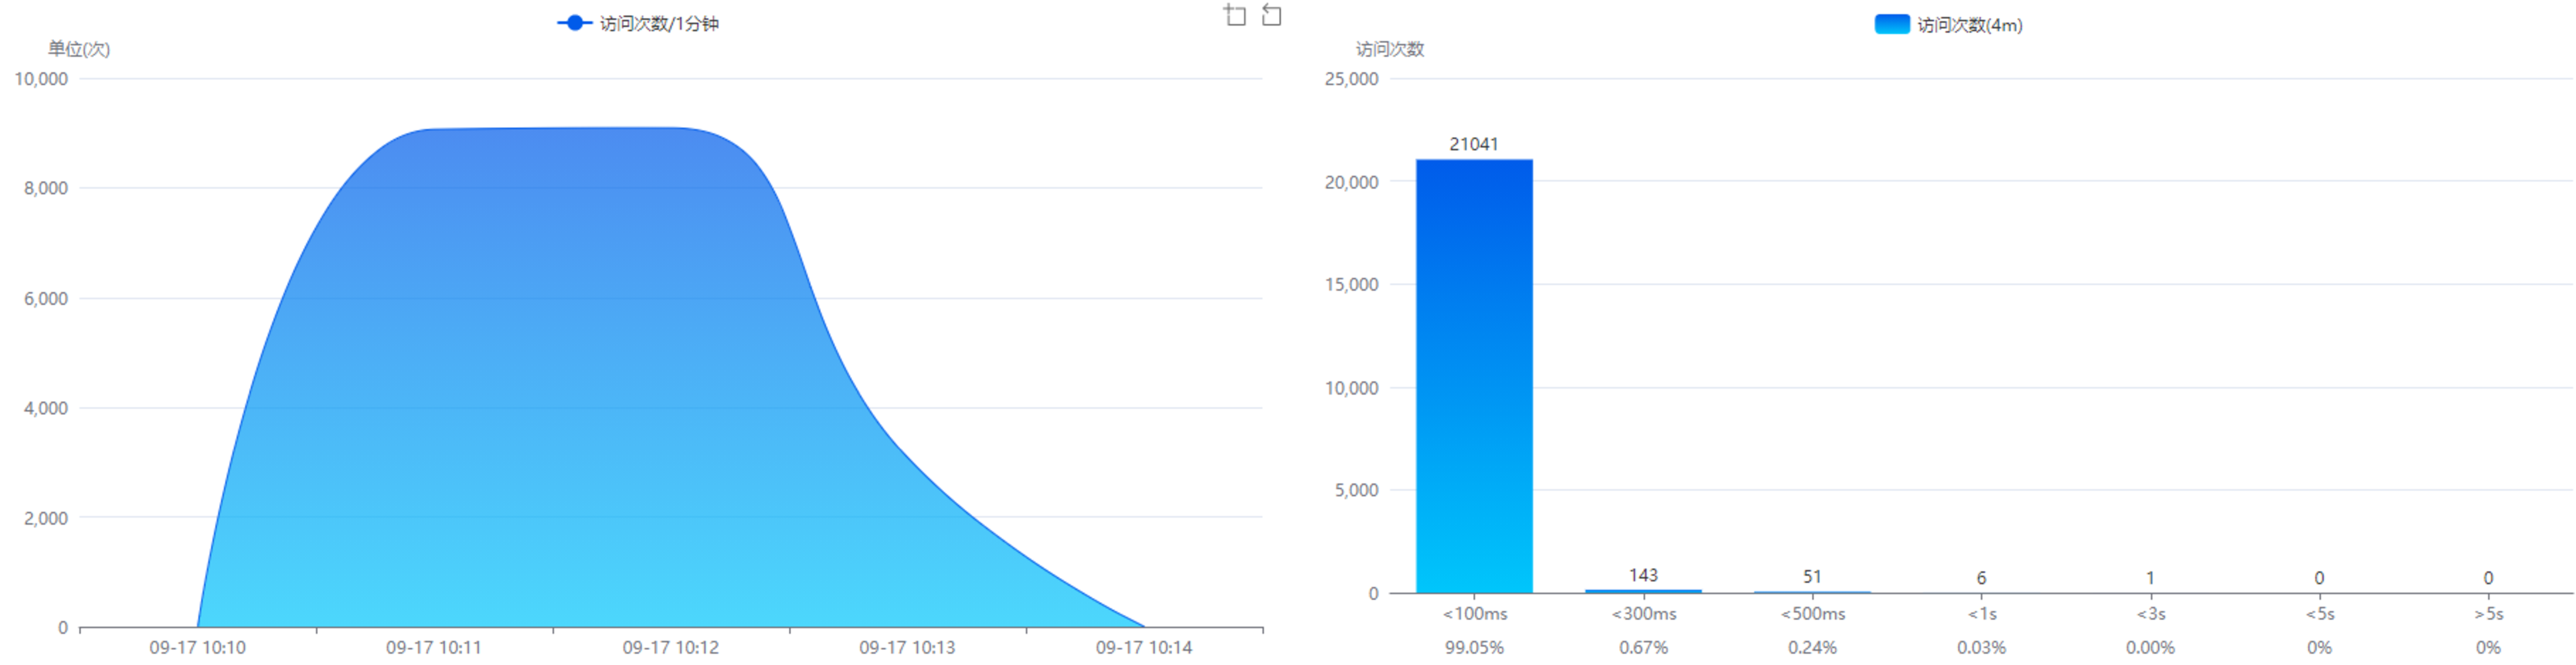
\includegraphics[width=1\textwidth]{压测.pdf}
    \caption{压力测试图}
    \label{fig:pressure}
\end{figure}


\subsection{易用性测试}

为了满足易用性测试,本系统在提供给用户使用时用户不需要关心数据库以
及前端页面的具体实现,用户只需根据自己的数据分析需求上传特定格式的文档即可,前端页面会自动渲染数据查询结果,以可视化的形式呈现数
据查询结果。因此发布的中文时间表达式信息抽取系统满足易用性的需求。

\subsection{兼容性测试}

为了满足兼容性测试,本系统的前端 Metis 页面分别在谷歌浏览器、Edge
浏览器、火狐浏览器、360 浏览器进行了测试,以上浏览器均能在 Metis 页面
上呈现功能测试中的各项数据,因此中文时间表达式信息抽取系统对以上各种
浏览器兼容。

\subsection{可维护性测试}

软件系统的可维护性可以用模块之间的耦合度、单元测试和集成测试的覆盖
率、代码规范等指标度量。本系统在开发过程中采用面向对象的设计方法,严格
遵循单一责任、低耦合高内聚等原则来进行系统模块的设计,减少模块与模块之
间的耦合度、增加模块内部的功能复用。系统在开发过程中也会在关键代码处添
加日志,当异常和错误情况发生时,开发人员能够快速通过日志进行问题解决。
综合以上分析,以太坊数据高速抽取和分析系统满足可维护性需求。


% !TeX root = ../main.tex

\chapter{总结与展望}

本章主要用来总结论文所做工作,在项目中的创新点和技术难点,并给出未来工作的展望和应该补足的一些工作。

本中文时间表达式识别与解析算法还具有一定的创新性,基于概率上下文无关语法,并应用全新的时间表达式的组合语义标注,以此来构建中文时间信息抽取系统;
此外,基于概率上下文无关语法,摆脱了完全基于规则,即使用正则表达式识别文本中的时间时,撰写规则的繁琐程度,同时用统计学的方法解决时间表达式识别中存在的冲突问题,识别结果更具有鲁棒性;
最后,应用时间表达式的组合语义标注,改良了 ISO-TimeML Timex3 标注格式的局限性,拓宽了时间表达式归一化后的语义表示范围。
除了核心算法的设计之外,本项目还将算法作为工具的一部分,完成了与后端交互的逻辑,即将算法组件作为外观模式层,完成与服务层的交互,同时为系统设计了一套用户交互界面和开发人用可应用编程接口,
方便用户使用和开发人员二次开发。 该项目已经能初步交付使用。

项目结束后,仍然不能算一个完全品,究其原因,在于基于概率无关的上下文语法仍然有一些问题无法解决:
\begin{enumerate}
    \item[(1)] 目前的研究中尚无将中文时间表达式作为语法来识别,现采用的概率上下文无关语法
    虽然能简化规则的撰写,但大量的语法规则的编写还是需要手工完成;
    \item[(2)] 语料库的缺乏会降低时间表达式归一化过程的准确度(Precision),主要体现为同一时
    间表达式解析出的多棵语法树间概率分布与真实数据分布不相匹配,当前还需要解决语料缺
    乏的问题;
    \item[(3)] 中文时间表达式归一化过程采用的 SCATE 结构与英语语境下的时间表达式相差比较
    大,需要重新设计以契合中文语境,此外,最终获得根结点上的嵌套表达式的计算方式,也需
    要重新设计。
\end{enumerate}

自笔者初步完成论文草稿时,自然语言处理中的时间表达式识别与解析的进展只能算小有进步。
中文时间表达式识别与解析影响较大的工作还时停留在2017年的论文中。 有关中文时间表达式识别与解析的研究道阻且长。


% % !TeX root = ../main.tex

\chapter{浮动体}

\section{三线表}

三线表是《撰写手册》推荐使用的格式,如表~\ref{tab:exampletable}。
\begin{table}[h]
  \centering
  \caption{表号和表题在表的正上方}
  \label{tab:exampletable}
  \begin{tabular}{cl}
    \toprule
    类型   & 描述                                       \\
    \midrule
    挂线表 & 挂线表也称系统表、组织表,用于表现系统结构 \\
    无线表 & 无线表一般用于设备配置单、技术参数列表等   \\
    卡线表 & 卡线表有完全表,不完全表和三线表三种       \\
    \bottomrule
  \end{tabular}
  \note{注:表注分两种,第一种是对全表的注释,用不加阿拉伯数字排在表的下边,
    前面加“注:”;第二种是和表内的某处文字或数字相呼应的注,
    在表里面用带圈的阿拉伯数字在右上角标出,然后在表下面用同样的圈码注出来}
\end{table}

编制表格应简单明了,表达一致,明晰易懂,表文呼应、内容一致。
排版时表格字号略小,或变换字体,尽量不分页,尽量不跨节。
表格太大需要转页时,需要在续表上方注明“续表”,表头页应重复排出。



\section{插图}

有的同学可能听说“\LaTeX{} 只能使用 eps 格式的图片”,甚至把 jpg 格式转为 eps。
事实上,这种做法已经过时。
而且每次编译时都要要调用外部工具解析 eps,导致降低编译速度。
所以我们推荐矢量图直接使用 pdf 格式,位图使用 jpeg 或 png 格式。
\begin{figure}[h]
  \centering
  \includegraphics[width=0.3\textwidth]{ustc-badge.pdf}
  \caption{图号、图题置于图的下方}
  \label{fig:badge}
  \note{注:图注的内容不宜放到图题中。}
\end{figure}

关于图片的并排,推荐使用较新的 \pkg{subcaption} 宏包,
不建议使用 \pkg{subfigure} 或 \pkg{subfig} 等宏包。



\section{算法环境}

模板中使用 \pkg{algorithm2e} 宏包实现算法环境。关于该宏包的具体用法,
请阅读宏包的官方文档。

\begin{algorithm}[h]
  \SetAlgoLined
  \KwData{this text}
  \KwResult{how to write algorithm with \LaTeX2e }

  initialization\;
  \While{not at end of this document}{
    read current\;
    \eIf{understand}{
      go to next section\;
      current section becomes this one\;
    }{
      go back to the beginning of current section\;
    }
  }
  \caption{算法示例1}
  \label{algo:algorithm1}
\end{algorithm}

注意,我们可以在论文中插入算法,但是插入大段的代码是愚蠢的。
然而这并不妨碍有的同学选择这么做,对于这些同学,建议用 \pkg{listings} 宏包。

% % !TeX root = ../main.tex

\chapter{数学}

\section{数学符号和公式}

《撰写手册》要求数学符号遵循 GB/T 3102.11—1993《物理科学和技术中使用的数学符号》
\footnote{原 GB 3102.11—1993,自 2017 年 3 月 23 日起,该标准转为推荐性标准。}。
该标准参照采纳 ISO 31-11:1992 \footnote{目前已更新为 ISO 80000-2:2019。},
但是与 \TeX{} 默认的美国数学学会(AMS)的符号习惯有所区别。
具体地来说主要有以下差异:
\begin{enumerate}
  \item 大写希腊字母默认为斜体,如
    \begin{equation*}
      \Gamma \Delta \Theta \Lambda \Xi \Pi \Sigma \Upsilon \Phi \Psi \Omega.
    \end{equation*}
    注意有限增量符号 $\increment$ 固定使用正体,模板提供了 \cs{increment} 命令。
  \item 小于等于号和大于等于号使用倾斜的字形 $\le$、$\ge$。
  \item 积分号使用正体,比如 $\int$、$\oint$。
  \item 行间公式积分号的上下限位于积分号的上下两端,比如
    \begin{equation*}
      \int_a^b f(x) \dif x.
    \end{equation*}
    行内公式为了版面的美观,统一居右侧,如 $\int_a^b f(x) \dif x$ 。
  \item
    偏微分符号 $\partial$ 使用正体。
  \item
    省略号 \cs{dots} 按照中文的习惯固定居中,比如
    \begin{equation*}
      1, 2, \dots, n \quad 1 + 2 + \dots + n.
    \end{equation*}
  \item
    实部 $\Re$ 和虚部 $\Im$ 的字体使用罗马体。
\end{enumerate}

以上数学符号样式的差异可以在模板中统一设置。
但是还有一些需要用户在写作时进行处理:
\begin{enumerate}
  \item 数学常数和特殊函数名用正体,如
    \begin{equation*}
      \uppi = 3.14\dots; \quad
      \symup{i}^2 = -1; \quad
      \symup{e} = \lim_{n \to \infty} \left( 1 + \frac{1}{n} \right)^n.
    \end{equation*}
  \item 微分号使用正体,比如 $\dif y / \dif x$。
  \item 向量、矩阵和张量用粗斜体(\cs{symbf}),如 $\symbf{x}$、$\symbf{\Sigma}$、$\symbfsf{T}$。
  \item 自然对数用 $\ln x$ 不用 $\log x$。
\end{enumerate}

模板中使用 \pkg{unicode-math} 宏包配置数学字体。
该宏包与传统的 \pkg{amsfonts}、\pkg{amssymb}、\pkg{bm}、
\pkg{mathrsfs}、\pkg{upgreek} 等宏包\emph{不}兼容。
本模板作了处理,用户可以直接使用 \cs{bm}, \cs{mathscr},
\cs{upGamma} 等命令。
关于数学符号更多的用法,参见 \pkg{unicode-math} 宏包的使用说明和符号列表
\pkg{unimath-symbols}。



\section{量和单位}

宏包 \pkg{siunitx} 提供了更好的数字和单位支持:
\begin{itemize}
  \item \num{12345.67890}
  \item \num{.3e45}
  \item \si{kg.m.s^{-1}}
  \item \si{\micro\meter} $\si{\micro\meter}$
  \item \si{\ohm} $\si{\ohm}$
  \item \numlist{10;20}
  \item \numlist{10;20;30}
  \item \SIlist{0.13;0.67;0.80}{\milli\metre}
  \item \numrange{10}{20}
  \item \SIrange{10}{20}{\degreeCelsius}
\end{itemize}



\section{定理和证明}

示例文件中使用 \pkg{amsthm} 宏包配置了定理、引理和证明等环境。
用户也可以使用 \pkg{ntheorem} 宏包。

\begin{definition}
  If the integral of function $f$ is measurable and non-negative, we define
  its (extended) \textbf{Lebesgue integral} by
  \begin{equation}
    \int f = \sup_g \int g,
  \end{equation}
  where the supremum is taken over all measurable functions $g$ such that
  $0 \le g \le f$, and where $g$ is bounded and supported on a set of
  finite measure.
\end{definition}

\begin{assumption}
The communication graph is strongly connected.
\end{assumption}

\begin{example}
  Simple examples of functions on $\mathbb{R}^d$ that are integrable
  (or non-integrable) are given by
  \begin{equation}
    f_a(x) =
    \begin{cases}
      |x|^{-a} & \text{if } |x| \le 1, \\
      0        & \text{if } x > 1.
    \end{cases}
  \end{equation}
  \begin{equation}
    F_a(x) = \frac{1}{1 + |x|^a}, \qquad \text{all } x \in \mathbb{R}^d.
  \end{equation}
  Then $f_a$ is integrable exactly when $a < d$, while $F_a$ is integrable
  exactly when $a > d$.
\end{example}

\begin{lemma}[Fatou]
  Suppose $\{f_n\}$ is a sequence of measurable functions with $f_n \geq 0$.
  If $\lim_{n \to \infty} f_n(x) = f(x)$ for a.e. $x$, then
  \begin{equation}
    \int f \le \liminf_{n \to \infty} \int f_n.
  \end{equation}
\end{lemma}

\begin{remark}
  We do not exclude the cases $\int f = \infty$,
  or $\liminf_{n \to \infty} f_n = \infty$.
\end{remark}

\begin{corollary}
  Suppose $f$ is a non-negative measurable function, and $\{f_n\}$ a sequence
  of non-negative measurable functions with
  $f_n(x) \le f(x)$ and $f_n(x) \to f(x)$ for almost every $x$. Then
  \begin{equation}
    \lim_{n \to \infty} \int f_n = \int f.
  \end{equation}
\end{corollary}

\begin{proposition}
  Suppose $f$ is integrable on $\mathbb{R}^d$. Then for every $\epsilon > 0$:
  \begin{enumerate}
    \renewcommand{\theenumi}{\roman{enumi}}
    \item There exists a set of finite measure $B$ (a ball, for example) such
      that
      \begin{equation}
        \int_{B^c} |f| < \epsilon.
      \end{equation}
    \item There is a $\delta > 0$ such that
      \begin{equation}
        \int_E |f| < \epsilon \qquad \text{whenever } m(E) < \delta.
      \end{equation}
  \end{enumerate}
\end{proposition}

\begin{theorem}
  Suppose $\{f_n\}$ is a sequence of measurable functions such that
  $f_n(x) \to f(x)$ a.e. $x$, as $n$ tends to infinity.
  If $|f_n(x)| \le g(x)$, where $g$ is integrable, then
  \begin{equation}
    \int |f_n - f| \to 0 \qquad \text{as } n \to \infty,
  \end{equation}
  and consequently
  \begin{equation}
    \int f_n \to \int f \qquad \text{as } n \to \infty.
  \end{equation}
\end{theorem}

\begin{proof}
  Trivial.
\end{proof}

\newtheorem*{axiomofchoice}{Axiom of choice}
\begin{axiomofchoice}
  Suppose $E$ is a set and ${E_\alpha}$ is a collection of
  non-empty subsets of $E$. Then there is a function $\alpha
  \mapsto x_\alpha$ (a ``choice function'') such that
  \begin{equation}
    x_\alpha \in E_\alpha,\qquad \text{for all }\alpha.
  \end{equation}
\end{axiomofchoice}

\newtheorem{observation}{Observation}
\begin{observation}
  Suppose a partially ordered set $P$ has the property
  that every chain has an upper bound in $P$. Then the
  set $P$ contains at least one maximal element.
\end{observation}
\begin{proof}[A concise proof]
  Obvious.
\end{proof}

% % !TeX root = ../main.tex

\chapter{引用文献的标注}

模板使用 \pkg{natbib} 宏包来设置参考文献引用的格式,
更多引用方法可以参考该宏包的使用说明。



\section{顺序编码制}

\subsection{角标数字标注法}

\ustcsetup{
  cite-style = super,
}
\noindent
\begin{tabular}{l@{\quad$\Rightarrow$\quad}l}
  \verb|\cite{knuth86a}| & \cite{knuth86a}         \\
  \verb|\citet{knuth86a}| & \citet{knuth86a}        \\
  \verb|\cite[42]{knuth86a}| & \cite[42]{knuth86a}     \\
  \verb|\cite{knuth86a,tlc2}| & \cite{knuth86a,tlc2}    \\
  \verb|\cite{knuth86a,knuth84}| & \cite{knuth86a,knuth84} \\
\end{tabular}


\subsection{数字标注法}

\ustcsetup{
  cite-style = inline,
}
\noindent
\begin{tabular}{l@{\quad$\Rightarrow$\quad}l}
  \verb|\cite{knuth86a}|  & \cite{knuth86a}         \\
  \verb|\citet{knuth86a}|  & \citet{knuth86a}        \\
  \verb|\cite[42]{knuth86a}|  & \cite[42]{knuth86a}     \\
  \verb|\cite{knuth86a,tlc2}|  & \cite{knuth86a,tlc2}    \\
  \verb|\cite{knuth86a,knuth84}| & \cite{knuth86a,knuth84} \\
\end{tabular}



\section{著者-出版年制标注法}

\ustcsetup{
  cite-style = authoryear,
}
\noindent
\begin{tabular}{l@{\quad$\Rightarrow$\quad}l}
  \verb|\cite{knuth86a}| & \cite{knuth86a}         \\
  \verb|\citep{knuth86a}| & \citep{knuth86a}        \\
  \verb|\citet[42]{knuth86a}| & \citet[42]{knuth86a}    \\
  \verb|\citep[42]{knuth86a}| & \citep[42]{knuth86a}    \\
  \verb|\cite{knuth86a,tlc2}| & \cite{knuth86a,tlc2}    \\
  \verb|\cite{knuth86a,knuth84}| & \cite{knuth86a,knuth84} \\
\end{tabular}

\ustcsetup{
  cite-style = super,
}

% 注意,参考文献列表中的每条文献在正文中都要被引用。这里只是为了示例。
\nocite{*}


\backmatter
\bibliography{bib/ustc}  % 参考文献使用 BibTeX 编译
% \printbibliography       % 参考文献使用 BibLaTeX 编译

% \appendix
% % !TeX root = ../main.tex

\chapter{补充材料}


\section{补充章节}

补充内容。


% !TeX root = ../main.tex

\begin{acknowledgements}

时间如白驹过隙, 入学的情景仿佛还在眼前, 中科大的研究生生活却要告一段落了.

首先要感谢我的指导老师王超老师和郭燕博士, 郭燕老师是我在自然语言处理领域的引路人, 当我选择放弃自然语言处理转向后端开发时, 
又是郭燕老师给予我指导, 让我快速的转换研究方向. 休学的这一年里, 郭燕老师给予我无微不至的关怀和鼓励, 让几度想要退学, 踌躇不前的我还是下定决心完成学业, 从事互联网行业的软件开发工作.
郭燕老师的人格魅力和无私精神我将永记于心, 我衷心的祝愿郭燕老师永远健康幸福, 工作顺利.

其次要感谢的我的企业导师詹恂昊(Hunt)工程师. Hunt不仅教会我自然语言处理的相关知识, 也让我知道怎样才算一名合格的软件开发工程师.
Hunt为我的职业生涯打下了良好的基础, 即使毕业后成为了一名后端工程师, Hunt的代码风格和极客精神永远值得我学习和追赶, 我对Hunt心怀感激.

再次要感谢308实验室的小伙伴们, 在308这间不大不小的实验室里, 碰撞出了许多思想的火花, 和小伙伴们一起讨论的时光是我美好的回忆, 跨领域和方向的交流让我大开眼界.
休学时也是你们鼓励我, 让我知道前路并非晦暗无光, 谢谢你们陪我一起度过这几年时光, 祝愿各位小伙伴们都前程似锦. 同时特别感谢江明燕同学给我的论文提出的修改意见.
感谢李春元同学参与了部分的实验设计.

最后, 感谢我的家人和朋友们, 休学这一年里他们在背后一直默默鼓励和支持我, 鼓励我走出困境. 感谢我的父母, 祝他们身体健康.

\end{acknowledgements}

% % !TeX root = ../main.tex

\begin{publications}

\section*{已发表论文}

\begin{enumerate}
\item A A A A A A A A A
\item A A A A A A A A A
\item A A A A A A A A A
\end{enumerate}

\section*{待发表论文}

\begin{enumerate}
\item A A A A A A A A A
\item A A A A A A A A A
\item A A A A A A A A A
\end{enumerate}

\section*{研究报告}
\begin{enumerate}
\item A A A A A A A A A
\item A A A A A A A A A
\item A A A A A A A A A
\end{enumerate}

\end{publications}


\end{sloppypar}
\end{document}
